% ============================================================================
% Rapport de mini-projet --- Industrie 4.0
% « Jumeau numérique d'une ligne de production »
% Auteurs    : A. Issami, M. Ezbakhe, H. Benzahra, Z. Hsain, H. Kichchou, M. Hamdouch
% Encadrante : Prof. Maria Zemzami (ENSAM Rabat)
% ENSAM Rabat --- Filière INDIA&SD --- Année Universitaire 2026/2027
% Compilation : make   (ou : pdflatex, bibtex, pdflatex, pdflatex)
% ============================================================================

\documentclass[12pt,a4paper,openany]{report}

% ============================================================================
% Préambule --- Rapport de mini-projet « Jumeau numérique d'une ligne de production »
% ENSAM Rabat --- Filière INDIA&SD --- Industrie 4.0 --- Année Universitaire 2026/2027
% Gabarit repris du rapport de stage PIPER Speech (même charte : bleu marine ENSAM).
% ============================================================================

\usepackage[utf8]{inputenc}
\usepackage[T1]{fontenc}
\usepackage[french]{babel}
\usepackage{lmodern}
\usepackage{geometry}
\usepackage{graphicx}
\usepackage{listings}
\usepackage{xcolor}
\usepackage{hyperref}
\usepackage{fancyhdr}
\usepackage{titlesec}
\usepackage{booktabs}
\usepackage{tabularx}
\usepackage{longtable}
\usepackage{enumitem}
\usepackage{tikz}
\usepackage{float}
\usepackage{amsmath}
\usepackage{amssymb}
\usepackage{caption}
\usepackage{subcaption}
\usepackage{tcolorbox}
\usepackage{acronym}
\usepackage{csquotes}
\usepackage{colortbl}
\usepackage{multirow}
\usepackage{pgfplots}
\pgfplotsset{compat=1.18}

\usetikzlibrary{shapes.geometric, arrows.meta, positioning, fit, backgrounds, calc}

% ---------------------------- Mise en page ----------------------------------
\geometry{a4paper, margin=2.5cm, headheight=15pt}

% Couleur principale : bleu marine académique ENSAM (identique au rapport PIPER),
% couleur secondaire : rouge du logo ENSAM.
\definecolor{ensambleu}{HTML}{1B3A5C}
\definecolor{ensamrouge}{HTML}{B22A2E}
\definecolor{lienviolet}{HTML}{4A148C}
\definecolor{etatmarche}{HTML}{22C55E}
\definecolor{etatattente}{HTML}{94A3B8}
\definecolor{etatbloque}{HTML}{F59E0B}
\definecolor{etatpanne}{HTML}{EF4444}

\hypersetup{
    colorlinks=true,
    linkcolor=lienviolet,
    urlcolor=lienviolet,
    citecolor=lienviolet,
    pdftitle={Jumeau numérique d'une ligne de production},
    pdfauthor={Issami, Ezbakhe, Benzahra, Hsain, Kichchou, Hamdouch}
}

% ---------------------------- Listings (code) -------------------------------
\definecolor{codebg}{HTML}{F5F5F5}
\definecolor{codegreen}{HTML}{28A745}
\definecolor{codepurple}{HTML}{6F42C1}
\definecolor{codegray}{HTML}{6A737D}

\lstdefinestyle{mystyle}{
    backgroundcolor=\color{codebg},
    commentstyle=\color{codegray}\itshape,
    keywordstyle=\color{codepurple}\bfseries,
    numberstyle=\tiny\color{codegray},
    stringstyle=\color{codegreen},
    basicstyle=\ttfamily\footnotesize,
    breakatwhitespace=false,
    breaklines=true,
    captionpos=b,
    keepspaces=true,
    numbers=left,
    numbersep=5pt,
    showspaces=false,
    showstringspaces=false,
    showtabs=false,
    tabsize=2,
    frame=single,
    rulecolor=\color{gray!30},
    extendedchars=true,
    inputencoding=utf8,
    literate=%
      {é}{{\'e}}1 {è}{{\`e}}1 {ê}{{\^e}}1 {ë}{{\"e}}1
      {à}{{\`a}}1 {â}{{\^a}}1 {ä}{{\"a}}1
      {î}{{\^i}}1 {ï}{{\"i}}1
      {ô}{{\^o}}1 {ö}{{\"o}}1
      {ù}{{\`u}}1 {û}{{\^u}}1 {ü}{{\"u}}1
      {ç}{{\c c}}1 {Ç}{{\c C}}1
      {É}{{\'E}}1 {È}{{\`E}}1 {À}{{\`A}}1 {×}{{$\times$}}1
}
\lstset{style=mystyle}

% ---------------------------- En-tête / pied --------------------------------
\renewcommand{\chaptermark}[1]{\markboth{\chaptername\ \thechapter}{}}

\pagestyle{fancy}
\fancyhf{}
\fancyhead[L]{\small\nouppercase{\leftmark}}
\fancyhead[R]{\small Jumeau numérique --- Industrie 4.0}
\fancyfoot[L]{\footnotesize ENSAM Rabat --- Année Universitaire 2026/2027}
\fancyfoot[R]{\thepage}
\renewcommand{\headrulewidth}{0.4pt}
\renewcommand{\footrulewidth}{0.4pt}

\fancypagestyle{plain}{%
  \fancyhf{}%
  \fancyfoot[L]{\footnotesize ENSAM Rabat --- Année Universitaire 2026/2027}%
  \fancyfoot[R]{\thepage}%
  \renewcommand{\headrulewidth}{0pt}%
  \renewcommand{\footrulewidth}{0.4pt}%
}

% ---------------------------- Titres chapitres ------------------------------
\titleformat{\chapter}[display]
  {\normalfont\huge\bfseries\color{ensambleu}}
  {\chaptertitlename\ \thechapter}{20pt}{\Huge}
\titlespacing*{\chapter}{0pt}{-20pt}{30pt}

% ---------------------------- Légendes --------------------------------------
\captionsetup{font=small, labelfont=bf, labelsep=period}

% ---------------------------- Macros utiles ---------------------------------
\newcommand{\produit}{\textbf{jumeau numérique}}
\newcommand{\code}[1]{\texttt{#1}}

\newtcolorbox{callout}[1][]{colback=ensambleu!5, colframe=ensambleu, sharp corners,
  boxrule=0.5pt, left=8pt, right=8pt, top=6pt, bottom=6pt, #1}
\newtcolorbox{success}[1][]{colback=green!6, colframe=green!60!black, sharp corners,
  boxrule=0.5pt, left=8pt, right=8pt, top=6pt, bottom=6pt, #1}
\newtcolorbox{warn}[1][]{colback=orange!6, colframe=orange!70!black, sharp corners,
  boxrule=0.5pt, left=8pt, right=8pt, top=6pt, bottom=6pt, #1}

\setlist[itemize]{itemsep=2pt, topsep=3pt}
\setlist[enumerate]{itemsep=2pt, topsep=3pt}

% ---------------------------- Acronymes -------------------------------------
\acrodef{3D}{Trois dimensions}
\acrodef{API}{Application Programming Interface}
\acrodef{CSV}{Comma-Separated Values}
\acrodef{ENSAM}{École Nationale Supérieure d'Arts et Métiers}
\acrodef{ERP}{Enterprise Resource Planning}
\acrodef{IHM}{Interface Homme-Machine}
\acrodef{INDIA}[INDIA\&SD]{Ingénierie Numérique en Data Science, Intelligence Artificielle \& Santé Digitale}
\acrodef{IoT}{Internet of Things}
\acrodef{JSON}{JavaScript Object Notation}
\acrodef{KPI}{Key Performance Indicator}
\acrodef{MES}{Manufacturing Execution System}
\acrodef{MTBF}{Mean Time Between Failures}
\acrodef{MTTR}{Mean Time To Repair}
\acrodef{OPC}[OPC UA]{Open Platform Communications Unified Architecture}
\acrodef{PLC}{Programmable Logic Controller}
\acrodef{REST}{Representational State Transfer}
\acrodef{SQL}{Structured Query Language}
\acrodef{TRS}{Taux de Rendement Synthétique}
\acrodef{WIP}{Work In Progress (en-cours)}
\acrodef{WS}{WebSocket}

\endinput


\begin{document}

% ============================================================================
% Page de garde --- même structure que le rapport PIPER Speech
% Deux logos : ENSAM (gauche) + Université Mohammed V (droite).
% ============================================================================

\begin{titlepage}
    \centering

    \begin{minipage}[c]{0.2\textwidth}
        \centering
        
\includegraphics[height=2.2cm]{images/logo_ensam.png}
    \end{minipage}\hfill
    \begin{minipage}[c]{0.56\textwidth}
        \centering
        {\normalsize\textbf{Université Mohammed V de Rabat}}\\[0.15cm]
        {\small École Nationale Supérieure d'Arts et Métiers}
    \end{minipage}\hfill
    \begin{minipage}[c]{0.2\textwidth}
        \centering
        
\includegraphics[height=2.2cm]{images/logo_um5.png}
    \end{minipage}\\[0.35cm]
    {\color{ensambleu}\rule{\textwidth}{0.8pt}}

    \vfill

    {\small F\,I\,L\,I\,È\,R\,E}\\[0.35cm]
    {\fontsize{50}{56}\selectfont\bfseries\textcolor{ensambleu}{INDIA\&SD}}\\[0.35cm]
    {\fontsize{20}{27}\selectfont\bfseries\textcolor{ensambleu}{Ingénierie Numérique en Data Science,\\ Intelligence Artificielle \& Santé Digitale}\par}

    \vfill

    {\color{ensambleu}\rule{\textwidth}{0.8pt}}\\[0.45cm]
    {\normalsize\bfseries R\,A\,P\,P\,O\,R\,T\quad D\,E\quad M\,I\,N\,I\,-\,P\,R\,O\,J\,E\,T}\\[0.15cm]
    {\small Industrie 4.0}\\[0.4cm]
    {\fontsize{24}{31}\selectfont\bfseries\textcolor{ensambleu}{Jumeau numérique\\ d'une ligne de production}\par}\vspace{0.4cm}
    {\normalsize Simuler le comportement d'une ligne, la superviser en temps réel\\[0.05cm]
     et tester virtuellement des scénarios d'optimisation}\\[0.35cm]
    {\color{ensambleu}\rule{\textwidth}{0.8pt}}\\[0.3cm]
    {\small\itshape Projet n\textsuperscript{o}\,3 de la liste \enquote{Projets dans le cadre de la thématique Industrie 4.0}}

    \vfill

    \begin{minipage}[t]{0.5\textwidth}
        \centering
        {\normalsize\textbf{Réalisé par}}\\[0.2cm]
        Aymane \textsc{Issami}\\[0.05cm]
        Marouan \textsc{Ezbakhe}\\[0.05cm]
        Hiba \textsc{Benzahra}\\[0.05cm]
        Zaid \textsc{Hsain}\\[0.05cm]
        Houssam \textsc{Kichchou}\\[0.05cm]
        Mohamed \textsc{Hamdouch}
    \end{minipage}\hfill
    \begin{minipage}[t]{0.46\textwidth}
        \centering
        {\normalsize\textbf{Encadré par}}\\[0.2cm]
        Prof. Maria \textsc{Zemzami} {\small (ENSAM)}
    \end{minipage}

    \vfill

    {\color{ensambleu}\rule{\textwidth}{0.8pt}}\\[0.2cm]
    {\small 3\textsuperscript{ème} année, S5 --- Année universitaire 2026/2027}

\end{titlepage}


\pagenumbering{roman}

\chapter*{Remerciements}
\addcontentsline{toc}{chapter}{Remerciements}
\thispagestyle{plain}

Au terme de ce mini-projet, nous tenons à remercier toutes les personnes qui ont contribué à sa réalisation.

Nos premiers remerciements s'adressent à \textbf{Prof. Maria Zemzami}, qui a proposé et encadré ce projet dans le cadre de la thématique Industrie~4.0. Son cahier des charges --- contexte et objectifs, spécifications fonctionnelles et techniques, aspects organisationnels et humains, livrables, planning et critères d'évaluation --- a structuré notre démarche du début à la fin, et ce rapport en reprend volontairement le plan.

Nous remercions également le corps professoral de l'École Nationale Supérieure d'Arts et Métiers (\ac{ENSAM}) de Rabat, et particulièrement les enseignants de la filière \textit{INDIA\&SD}, pour la qualité de la formation dispensée~: les compétences en programmation, en modélisation et en analyse de données acquises au cours de notre cursus ont été mobilisées à chaque étape du projet.

Enfin, chaque membre de l'équipe remercie les cinq autres pour la rigueur et l'entraide dont chacun a fait preuve~: un jumeau numérique n'existe que si la simulation, la communication, la \ac{3D} et le tableau de bord parlent le même langage, et cet accord s'est construit ensemble.

\vspace{1.5cm}
\begin{flushright}
\textit{A.~\textsc{Issami}, M.~\textsc{Ezbakhe}, H.~\textsc{Benzahra},}\\
\textit{Z.~\textsc{Hsain}, H.~\textsc{Kichchou}, M.~\textsc{Hamdouch}}\\
\textit{2026}
\end{flushright}

\clearpage
\chapter*{Résumé}
\addcontentsline{toc}{chapter}{Résumé}
\thispagestyle{plain}

Ce rapport présente la conception et la réalisation d'un \textbf{jumeau numérique d'une ligne de production simplifiée}, dans le cadre du mini-projet Industrie~4.0 de l'\ac{ENSAM} Rabat. La ligne étudiée comporte quatre postes successifs --- alimentation (5~s), traitement (8~s), contrôle qualité (15~s) et emballage (7~s) --- reliés par un convoyeur, avec des files d'attente de capacité limitée, des pannes aléatoires et un taux de rejet de 5~\% au contrôle.

Le système repose sur une architecture en trois briques. Un \textbf{modèle de simulation} écrit en Python reproduit le comportement de la ligne par pas de temps de 0{,}05~s~: états des machines (en marche, en attente, bloquée, en panne), blocages de l'amont, propagation des pannes et calcul des \ac{KPI}. Un \textbf{backend} FastAPI diffuse l'état complet de la ligne dix fois par seconde par \ac{WS}, reçoit les commandes de l'opérateur et enregistre l'historique de production dans une base SQLite. Une \textbf{interface} web affiche la ligne en \ac{3D} avec une scène Unity exportée en WebGL et un tableau de bord de supervision synchronisé sur le même flux de données.

Le scénario d'optimisation porte sur le goulot d'étranglement du contrôle qualité. Sur une heure simulée avec pannes et une graine aléatoire identique pour tous les scénarios, la ligne initiale produit \textbf{218 produits}. Un contrôle automatisé à 8~s ou un second poste de contrôle en parallèle portent la production à \textbf{393} et \textbf{394 produits} (+80~\%), divisent l'attente au contrôle par 9 à 13 et déplacent le goulot vers le poste de traitement. Ces résultats sont mesurés avec la scène Unity connectée au backend. Un convoyeur adaptatif ne change pas le débit mais réduit l'en-cours moyen de 51~\%. La cohérence du modèle est vérifiée par 23 tests automatisés (débit de régime égal au débit théorique à 5~\% près, conservation des produits, capacité des files, effet des pannes). Les limites --- données entièrement simulées, absence de connexion à des équipements réels --- sont discutées en conclusion.

\vspace{0.4cm}
\textbf{Mots-clés~:} Industrie~4.0, jumeau numérique, simulation de ligne de production, goulot d'étranglement, supervision temps réel, WebSocket, Unity, WebGL, indicateurs de performance.

\vspace{1.2cm}

\chapter*{Abstract}
\addcontentsline{toc}{chapter}{Abstract}
\thispagestyle{plain}

This report presents the design and implementation of a \textbf{digital twin of a simplified production line}, carried out as part of the Industry~4.0 mini-project at \ac{ENSAM} Rabat. The line has four successive stations --- feeding (5~s), processing (8~s), quality control (15~s) and packaging (7~s) --- linked by a conveyor, with limited-capacity buffers, random breakdowns and a 5\% reject rate at quality control.

The system is built from three components. A \textbf{simulation model} written in Python reproduces the behaviour of the line in 0.05~s time steps: machine states (running, idle, blocked, down), upstream blocking, failure propagation and \ac{KPI} computation. A FastAPI \textbf{backend} streams the full line state ten times per second over \ac{WS}, receives operator commands and stores the production history in an SQLite database. A web \textbf{interface} renders the line in \ac{3D} with a Unity scene exported to WebGL, together with a supervision dashboard synchronised on the same data stream.

The optimisation scenario targets the quality-control bottleneck. Over one simulated hour with breakdowns and the same random seed for every scenario, the initial line produces \textbf{218 products}. An automated 8~s inspection or a second parallel inspection station raise output to \textbf{393} and \textbf{394 products} (+80\%), cut the waiting time at inspection by a factor of 9 to 13, and shift the bottleneck to the processing station. These results were measured with the Unity scene connected to the backend. An adaptive conveyor leaves throughput unchanged but reduces average work-in-progress by 51\%. Model consistency is checked by 23 automated tests (steady-state throughput within 5\% of theory, product conservation, buffer capacity, failure effects). The limitations --- fully simulated data, no connection to real equipment --- are discussed in the conclusion.

\vspace{0.4cm}
\textbf{Keywords:} Industry~4.0, digital twin, production line simulation, bottleneck, real-time supervision, WebSocket, Unity, WebGL, performance indicators.

\clearpage

\renewcommand{\contentsname}{Table des matières}
\tableofcontents
\clearpage
\listoffigures
\clearpage
\listoftables
\clearpage
\chapter*{Liste des acronymes}
\addcontentsline{toc}{chapter}{Liste des acronymes}
\thispagestyle{plain}

\begin{acronym}[Representational]
  \acro{3D}{Trois dimensions}
  \acro{API}{Application Programming Interface}
  \acro{CSV}{Comma-Separated Values}
  \acro{ENSAM}{École Nationale Supérieure d'Arts et Métiers}
  \acro{ERP}{Enterprise Resource Planning}
  \acro{IHM}{Interface Homme-Machine}
  \acro{INDIA}[INDIA\&SD]{Ingénierie Numérique en Data Science, Intelligence Artificielle \& Santé Digitale}
  \acro{IoT}{Internet of Things}
  \acro{JSON}{JavaScript Object Notation}
  \acro{KPI}{Key Performance Indicator}
  \acro{MES}{Manufacturing Execution System}
  \acro{MTBF}{Mean Time Between Failures}
  \acro{MTTR}{Mean Time To Repair}
  \acro{OPC}[OPC UA]{Open Platform Communications Unified Architecture}
  \acro{PLC}{Programmable Logic Controller}
  \acro{REST}{Representational State Transfer}
  \acro{SQL}{Structured Query Language}
  \acro{TRS}{Taux de Rendement Synthétique}
  \acro{WIP}{Work In Progress (en-cours)}
  \acro{WS}{WebSocket}
\end{acronym}

\clearpage

\pagenumbering{arabic}
\setcounter{page}{1}

% ============================================================================
% Introduction générale
% ============================================================================
\chapter*{Introduction générale}
\addcontentsline{toc}{chapter}{Introduction générale}
\markboth{Introduction générale}{}

Modifier une ligne de production réelle coûte cher~: chaque essai immobilise des machines, consomme de la matière et fait courir un risque sur la production. L'une des promesses de l'Industrie~4.0 est de déplacer une partie de ces essais vers un modèle virtuel fidèle de l'installation, le \textbf{jumeau numérique}, alimenté par des données et capable de répondre à la question \enquote{que se passerait-il si~?} avant toute intervention physique.

Ce mini-projet, troisième sujet de la liste proposée par Prof.~Maria Zemzami~\cite{zemzami2026}, a pour objectif de \textbf{modéliser une ligne de production simplifiée sous forme de jumeau numérique, permettant de simuler son comportement et de tester des scénarios d'optimisation}. Trois livrables sont attendus~: un modèle de simulation du système physique, une interface synchronisée avec des données simulées, et un scénario d'optimisation testé et documenté.

Nous avons réalisé ces trois livrables sous la forme d'une application complète, développée à six et versionnée dans un dépôt Git~: une simulation Python de la ligne, un backend temps réel qui la diffuse par WebSocket et en conserve l'historique, une scène \ac{3D} réalisée avec Unity et exportée en WebGL, un tableau de bord de supervision, ainsi qu'un module de comparaison de scénarios et une suite de tests automatisés qui valident la cohérence du modèle. Les résultats d'optimisation présentés dans ce rapport ont été mesurés avec la scène Unity elle-même, connectée au backend.

Le rapport suit le plan du cahier des charges. Le chapitre~\ref{chap:contexte} situe le projet dans l'Industrie~4.0 et en fixe le périmètre et les objectifs. Le chapitre~\ref{chap:specs} détaille les spécifications fonctionnelles et techniques. Le chapitre~\ref{chap:conception} présente la conception (architecture, modèle de simulation, protocole d'échange, répartition des rôles), et le chapitre~\ref{chap:implementation} sa réalisation. Le chapitre~\ref{chap:optimisation} documente le scénario d'optimisation et ses résultats chiffrés. Le chapitre~\ref{chap:organisation} traite des aspects organisationnels et humains, et le chapitre~\ref{chap:conclusion} dresse le bilan, les limites assumées et les perspectives.

% ============================================================================
% Chapitre 1 --- Contexte et objectifs
% ============================================================================
\chapter{Contexte et objectifs du projet}
\label{chap:contexte}

\section{L'Industrie 4.0 en quelques mots}

Le terme \textit{Industrie~4.0} désigne la quatrième révolution industrielle, après la mécanisation (vapeur), la production de masse (électricité) et l'automatisation (électronique et informatique). Formalisée en Allemagne au début des années~2010~\cite{kagermann2013}, elle repose sur l'interconnexion des équipements de production, des systèmes d'information et des personnes~: les machines communiquent leur état, les données sont collectées et analysées en continu, et les décisions de pilotage s'appuient sur ces données plutôt que sur l'observation ponctuelle.

Parmi les technologies associées --- capteurs et objets connectés (\ac{IoT}), informatique en nuage, intelligence artificielle, réalité augmentée, robotique collaborative --- le \textbf{jumeau numérique} occupe une place centrale~\cite{tao2019}, parce qu'il relie toutes les autres~: il est la représentation numérique vivante de l'installation, sur laquelle on peut observer, analyser et expérimenter.

\section{Le jumeau numérique}

Le concept a été formulé par Michael Grieves au début des années~2000 dans le contexte de la gestion du cycle de vie des produits~\cite{grieves2014}~: un objet physique, son double virtuel, et le flux de données qui les relie. La littérature distingue trois niveaux d'intégration selon la nature de ce flux~\cite{kritzinger2018}~:

\begin{table}[H]
\centering
\caption{Les trois niveaux d'intégration selon Kritzinger et al.}
\label{tab:niveaux}
\begin{tabularx}{\textwidth}{@{}l X X@{}}
\toprule
\textbf{Niveau} & \textbf{Physique $\rightarrow$ numérique} & \textbf{Numérique $\rightarrow$ physique} \\
\midrule
Modèle numérique & Manuel & Manuel \\
Ombre numérique (\textit{digital shadow}) & Automatique & Manuel \\
Jumeau numérique (\textit{digital twin}) & Automatique & Automatique \\
\bottomrule
\end{tabularx}
\end{table}

Dans un contexte académique sans équipement physique, le système physique est lui-même remplacé par une simulation. Notre projet se situe donc à l'interface entre ces niveaux~: la \enquote{ligne} est un modèle de simulation qui joue le rôle du système réel et produit des données en continu, et le jumeau (scène \ac{3D} et tableau de bord) se synchronise automatiquement sur ces données et peut renvoyer des commandes (changement de réglage, panne provoquée, réparation) qui modifient le comportement de la ligne. C'est précisément ce que demande le livrable \enquote{interface synchronisée avec des données simulées}. La norme ISO~23247~\cite{iso23247} décrit un cadre de référence pour ces jumeaux numériques de fabrication, dont notre architecture reprend la séparation entre entité observée, collecte des données et applications utilisatrices.

\section{Périmètre du projet}

\begin{table}[H]
\centering
\caption{Périmètre du projet.}
\label{tab:perimetre}
\begin{tabularx}{\textwidth}{@{}X X@{}}
\toprule
\textbf{Inclus} & \textbf{Exclu} \\
\midrule
Ligne de 4 postes en série, convoyeur, files d'attente de capacité limitée & Connexion à des automates (\ac{PLC}) ou capteurs réels \\
Pannes aléatoires et provoquées, rejets au contrôle qualité & Maintenance prédictive par apprentissage automatique \\
Visualisation \ac{3D} animée et tableau de bord synchronisés & Gestion des stocks, de la planification et des commandes (\ac{ERP}, \ac{MES}) \\
Historique de production et export des données & Déploiement en production, authentification des utilisateurs \\
Scénarios d'optimisation comparés dans des conditions identiques & Optimisation économique (coûts, investissements) \\
\bottomrule
\end{tabularx}
\end{table}

\section{La ligne étudiée}

La ligne comprend quatre postes successifs~: \textbf{alimentation}, \textbf{traitement}, \textbf{contrôle qualité} et \textbf{emballage}. Les produits circulent sur un convoyeur et passent par chaque poste. Les temps de traitement de départ sont ceux de l'énoncé du scénario~:

\begin{table}[H]
\centering
\caption{Paramètres initiaux de la ligne.}
\label{tab:parametres}
\begin{tabular}{@{}lcc@{}}
\toprule
\textbf{Poste} & \textbf{Temps de traitement} & \textbf{Cadence maximale isolée} \\
\midrule
Alimentation & 5~s & 12 produits/min \\
Traitement & 8~s & 7{,}5 produits/min \\
Contrôle qualité & 15~s & \textbf{4 produits/min} \\
Emballage & 7~s & 8{,}6 produits/min \\
\bottomrule
\end{tabular}
\end{table}

Dans une ligne en série, le débit est limité par le poste le plus lent~: c'est le \textbf{goulot d'étranglement}, au sens de la théorie des contraintes~\cite{goldratt1984}. Ici, le contrôle qualité (15~s) borne la ligne à 4~produits/min, soit 240 produits/h, alors que les autres postes pourraient aller plus vite. Les produits s'accumulent devant lui et les postes amont finissent par se bloquer.

\section{Objectifs}

\begin{enumerate}
  \item \textbf{Modéliser} la ligne de façon suffisamment fidèle pour reproduire les phénomènes qui comptent pour la décision~: goulot, accumulation, blocage de l'amont, effet des pannes et des rejets.
  \item \textbf{Superviser} la ligne en temps réel dans une interface \ac{3D} et un tableau de bord qui affichent les mêmes données au même instant.
  \item \textbf{Optimiser}~: identifier le goulot, tester plusieurs solutions et mesurer leur effet sur le débit, l'attente et l'en-cours, dans des conditions comparables.
  \item \textbf{Valider} le modèle par des tests automatisés plutôt que par la seule observation visuelle.
\end{enumerate}

% ============================================================================
% Chapitre 2 --- Spécifications fonctionnelles et techniques
% ============================================================================
\chapter{Spécifications fonctionnelles et techniques}
\label{chap:specs}

\section{Spécifications fonctionnelles}

Le cahier des charges propose une liste de fonctionnalités possibles. Le tableau~\ref{tab:fonctionnel} indique comment chacune est couverte par le projet.

\begin{table}[H]
\centering
\caption{Couverture des fonctionnalités du cahier des charges.}
\label{tab:fonctionnel}
\begin{tabularx}{\textwidth}{@{}p{4.2cm} X c@{}}
\toprule
\textbf{Fonctionnalité} & \textbf{Réalisation dans le projet} & \textbf{Statut} \\
\midrule
Automatisation des processus & Enchaînement automatique des postes, transfert par convoyeur, blocage et reprise sans intervention & Réalisé \\
Collecte et analyse de données en temps réel & État complet diffusé 10~fois/s, \ac{KPI} calculés en continu, historique SQLite par minute simulée & Réalisé \\
Interconnexion des équipements et systèmes & Simulation, backend, scène \ac{3D} et tableau de bord reliés par un protocole \ac{WS} unique & Réalisé \\
Interface homme-machine intuitive & Scène \ac{3D} navigable, voyants d'état, tableau de bord, onglet d'aide, manuel utilisateur & Réalisé \\
Maintenance prédictive & Pannes simulées, \ac{MTBF} et \ac{MTTR} observés par poste~; pas de modèle prédictif & Partiel \\
\bottomrule
\end{tabularx}
\end{table}

Les fonctions détaillées attendues par l'utilisateur sont les suivantes~:

\begin{itemize}
  \item \textbf{F1 --- Visualiser} la ligne en \ac{3D}~: machines, convoyeur, produits en mouvement, état de chaque machine (en marche, en attente, bloquée, en panne), avancement du produit en cours.
  \item \textbf{F2 --- Superviser}~: cadence réelle et théorique, produits finis, rejets, en-cours, goulot, état et statistiques de chaque poste.
  \item \textbf{F3 --- Piloter}~: pause, vitesse de simulation ($\times$1 à $\times$20), remise à zéro, modification des temps de cycle, nombre de machines en parallèle, convoyeur adaptatif, activation des pannes.
  \item \textbf{F4 --- Simuler des incidents}~: provoquer ou réparer une panne sur un poste choisi.
  \item \textbf{F5 --- Comparer}~: simuler une heure de chaque scénario dans des conditions identiques et afficher les écarts par rapport à la situation initiale.
  \item \textbf{F6 --- Historiser}~: conserver chaque exécution, consulter ses courbes et événements, exporter les données en \ac{CSV}.
\end{itemize}

\section{Spécifications techniques}

\subsection{Technologies retenues}

\begin{table}[H]
\centering
\caption{Choix technologiques.}
\label{tab:techno}
\begin{tabularx}{\textwidth}{@{}l l X@{}}
\toprule
\textbf{Brique} & \textbf{Technologie} & \textbf{Justification} \\
\midrule
Simulation & Python 3.12 & Langage maîtrisé par toute l'équipe, lisible pour un modèle métier, sans dépendance \\
Backend & FastAPI + Uvicorn~\cite{fastapi} & Serveur asynchrone léger qui gère à la fois \ac{WS} et \ac{REST} \\
Communication & WebSocket~\cite{rfc6455} & Canal bidirectionnel persistant et à faible latence~: l'état descend, les commandes remontent \\
Stockage & SQLite & Base \ac{SQL} embarquée dans la bibliothèque standard, un seul fichier, aucun serveur \\
\ac{3D} & Unity~6 (URP), export WebGL~\cite{unity6} & Moteur de jeu standard de l'industrie pour les jumeaux numériques, rendu dans le navigateur sans installation côté poste opérateur \\
Tableau de bord & HTML, CSS, JavaScript & Même page que la scène Unity, relié au même backend~; le tableau de bord et la \ac{3D} reçoivent le même état \\
Validation & pytest & Tests automatisés reproductibles du modèle et de l'\ac{API} \\
\bottomrule
\end{tabularx}
\end{table}

\begin{callout}
\textbf{Pourquoi Unity avec export WebGL~?} Le plan de travail prévoyait Unity, moteur de référence pour les jumeaux numériques. Une première version de la scène avait été écrite avec Three.js~; nous l'avons reconstruite dans Unity pour respecter la consigne et obtenir un rendu plus réaliste (éclairage, matériaux, brouillard, ombres). Pour ne pas séparer la \ac{3D} du tableau de bord, la scène est exportée en \textbf{WebGL} et affichée dans la même page web que le tableau de bord~: le navigateur sert d'unique poste de supervision, sans installation. Un petit pont (\code{LineBridge}) relie la page et la scène (sélection d'une machine dans les deux sens). La contrepartie est un build plus lourd (environ 12~Mo) et un premier chargement de quelques secondes.
\end{callout}

\subsection{Normes et standards}

Le projet s'appuie sur des standards ouverts~: le protocole WebSocket (RFC~6455~\cite{rfc6455}) pour la communication, \ac{JSON} pour le format des messages, HTTP/\ac{REST} pour l'historique, \ac{CSV} pour l'export. Dans une version industrielle, la collecte des données machines passerait par \ac{OPC} (IEC~62541~\cite{opcua}), standard de fait de l'interopérabilité industrielle~; l'architecture actuelle isole la source de données dans un seul module (\code{sim.py}) précisément pour permettre ce remplacement.

\subsection{Sécurité et cybersécurité}

Le serveur écoute uniquement sur l'interface locale (\code{127.0.0.1})~: il n'est pas exposé au réseau. Les commandes reçues sont validées et bornées côté serveur (numéro de poste, temps de cycle entre 1 et 60~s, 1 à 3 machines, vitesse entre $\times$0{,}25 et $\times$20)~; une commande invalide renvoie un message d'erreur sans modifier l'état. Aucune donnée personnelle n'est traitée. Une mise en réseau réelle demanderait en plus une authentification des opérateurs, un chiffrement (\code{wss://}) et des droits différenciés entre consultation et pilotage~; ces points sont listés dans les perspectives.

\subsection{Performances attendues}

\begin{table}[H]
\centering
\caption{Exigences de performance et valeurs obtenues.}
\label{tab:perf}
\begin{tabularx}{\textwidth}{@{}X p{3.1cm} p{3.6cm}@{}}
\toprule
\textbf{Exigence} & \textbf{Cible} & \textbf{Obtenu} \\
\midrule
Fréquence de mise à jour de l'interface & $\geq$ 5~Hz & 10~Hz \\
Pas de simulation & $\leq$ 0{,}1~s & 0{,}05~s \\
Taille d'un message d'état & $<$ 10~ko & $\approx$ 3~ko \\
Comparaison de 5 scénarios sur 1~h simulée & $<$ 5~s & $\approx$ 0{,}3~s \\
Écart débit simulé / débit théorique en régime & $\leq$ 5~\% & vérifié par test \\
Écart entre la mesure avec la scène Unity et la simulation hors ligne & $\leq$ 2~\% & 1{,}3~\% au maximum \\
Rendu \ac{3D} & fluide (cible 30~images/s ou plus) & à mesurer sur le poste de démonstration \\
\bottomrule
\end{tabularx}
\end{table}

% ============================================================================
% Chapitre 3 --- Conception
% ============================================================================
\chapter{Conception du jumeau numérique}
\label{chap:conception}

\section{Architecture générale}

Le système est découpé en trois couches, représentées en figure~\ref{fig:architecture}~: la \textbf{ligne simulée}, qui joue le rôle du système physique~; le \textbf{backend}, qui la fait avancer, la diffuse et en garde la mémoire~; et l'\textbf{interface}, qui la représente et la pilote.

\begin{figure}[H]
\centering
\begin{tikzpicture}[
  box/.style={draw=ensambleu, fill=ensambleu!6, rounded corners=3pt, minimum width=3.4cm, minimum height=1.05cm, align=center, font=\small},
  db/.style={draw=ensamrouge, fill=ensamrouge!6, rounded corners=3pt, minimum width=3.4cm, minimum height=1.05cm, align=center, font=\small},
  grp/.style={draw=gray!60, dashed, rounded corners=6pt, inner sep=8pt},
  arr/.style={-{Stealth[length=2.5mm]}, thick, ensambleu},
  lbl/.style={font=\scriptsize, fill=white, inner sep=1.5pt}
]
\node[box] (scene) {\textbf{scene.js}\\ scène 3D Three.js};
\node[box, below=0.7cm of scene] (app) {\textbf{app.js}\\ tableau de bord, commandes};
\node[grp, fit=(scene)(app), label={[font=\small\bfseries]above:Navigateur (interface)}] (nav) {};

\node[box, right=4.2cm of scene] (server) {\textbf{server.py}\\ FastAPI, WebSocket, REST};
\node[box, below=0.7cm of server] (sim) {\textbf{sim.py}\\ modèle de la ligne, KPI};
\node[db, below=0.7cm of sim] (storage) {\textbf{storage.py}\\ historique SQLite};
\node[grp, fit=(server)(sim)(storage), label={[font=\small\bfseries]above:Backend Python}] (back) {};

\draw[arr] ([yshift=4pt]server.west) -- node[lbl, above=2pt]{état JSON, 10~Hz} ([yshift=4pt]nav.east |- server.west);
\draw[arr] ([yshift=-14pt]nav.east |- server.west) -- node[lbl, below=2pt]{commandes} ([yshift=-14pt]server.west);
\draw[arr, dashed] (app.east) -- node[lbl, below=2pt]{REST : historique, CSV} (app.east -| back.west);
\draw[arr] (server) -- node[lbl, right]{pas de 0,05 s} (sim);
\draw[arr] (sim) -- node[lbl, right]{1 relevé / min simulée} (storage);
\draw[arr] (app) -- node[lbl, left]{même message} (scene);
\end{tikzpicture}
\caption{Architecture du jumeau numérique.}
\label{fig:architecture}
\end{figure}

Le choix structurant est que \textbf{la scène \ac{3D} et le tableau de bord lisent le même message}. Le backend n'envoie pas une information à la \ac{3D} et une autre au tableau de bord~: il envoie un état unique de la ligne (machines, files, produits, \ac{KPI}), et chaque vue en extrait ce qu'elle affiche. Il est donc impossible que la \ac{3D} montre une machine en panne pendant que le tableau de bord la déclare en marche.

\section{Modèle de simulation de la ligne}

\subsection{Flux physique}

\begin{figure}[H]
\centering
\resizebox{\textwidth}{!}{%
\begin{tikzpicture}[
  st/.style={draw=ensambleu, fill=ensambleu, text=white, rounded corners=2pt, minimum width=2.1cm, minimum height=1cm, align=center, font=\small\bfseries},
  buf/.style={draw=gray!70, fill=gray!10, minimum width=1.1cm, minimum height=0.6cm, align=center, font=\scriptsize},
  arr/.style={-{Stealth[length=2mm]}, thick}
]
\node[st] (a) {Alimen-\\tation\\[-2pt]{\scriptsize 5 s}};
\node[buf, right=0.45cm of a] (b1) {file $\leq$ 8};
\node[st, right=0.45cm of b1] (t) {Traite-\\ment\\[-2pt]{\scriptsize 8 s}};
\node[buf, right=0.45cm of t] (b2) {file $\leq$ 8};
\node[st, fill=ensamrouge, draw=ensamrouge, right=0.45cm of b2] (c) {Contrôle\\qualité\\[-2pt]{\scriptsize 15 s}};
\node[buf, right=0.45cm of c] (b3) {file $\leq$ 8};
\node[st, right=0.45cm of b3] (e) {Embal-\\lage\\[-2pt]{\scriptsize 7 s}};
\draw[arr] (a) -- (b1); \draw[arr] (b1) -- (t); \draw[arr] (t) -- (b2); \draw[arr] (b2) -- (c);
\draw[arr] (c) -- (b3); \draw[arr] (b3) -- (e);
\draw[arr] (e.east) -- ++(0.6,0) node[right, font=\scriptsize]{produits finis};
\draw[arr, ensamrouge] (c.south) -- ++(0,-0.7) node[below, font=\scriptsize]{rejets (5~\%)};
\node[font=\scriptsize, gray, below=0.25cm of b1] {convoyeur 2 s};
\node[font=\scriptsize, gray, below=0.25cm of b3] {convoyeur 2 s};
\end{tikzpicture}}
\caption{Flux des produits dans la ligne modélisée.}
\label{fig:flux}
\end{figure}

L'alimentation dispose d'une matière première illimitée et produit dès qu'elle est libre. Chaque produit terminé est déposé sur le convoyeur (2~s de transfert) puis rejoint la file du poste suivant. Les files ont une \textbf{capacité de 8 produits}~: si la file aval, convoyeur compris, est pleine, le poste qui vient de terminer garde son produit et se \textbf{bloque}. C'est ce mécanisme qui propage un goulot ou une panne vers l'amont, comme sur une vraie ligne. Au contrôle qualité, chaque produit est rejeté avec une probabilité de 5~\% et retiré de la ligne.

\subsection{États d'une machine}

\begin{figure}[H]
\centering
\begin{tikzpicture}[
  s/.style={draw, circle, minimum size=1.9cm, align=center, font=\small\bfseries, line width=1pt},
  arr/.style={-{Stealth[length=2mm]}, thick},
  lbl/.style={font=\scriptsize, align=center}
]
\node[s, draw=etatattente, fill=etatattente!15] (att) {En\\attente};
\node[s, draw=etatmarche, fill=etatmarche!15, right=3cm of att] (mar) {En\\marche};
\node[s, draw=etatbloque, fill=etatbloque!15, right=3cm of mar] (blo) {Bloquée};
\node[s, draw=etatpanne, fill=etatpanne!15, below=1.6cm of mar] (pan) {En\\panne};
\draw[arr] (att) to[bend left=20] node[lbl, above]{produit disponible} (mar);
\draw[arr] (mar) to[bend left=20] node[lbl, below]{fini, file aval libre,\\pas de produit en amont} (att);
\draw[arr] (mar) to[bend left=20] node[lbl, above]{fini, file aval pleine} (blo);
\draw[arr] (blo) to[bend left=20] node[lbl, below]{place libérée} (mar);
\draw[arr] ([xshift=-4pt]mar.south) to[bend right=25] node[lbl, left=2pt]{panne\\(MTBF)} ([xshift=-4pt]pan.north);
\draw[arr] ([xshift=4pt]pan.north) to[bend right=25] node[lbl, right=2pt]{réparation\\(MTTR)} ([xshift=4pt]mar.south);
\end{tikzpicture}
\caption{Machine à états d'un poste (le voyant de la scène 3D reprend ces quatre couleurs).}
\label{fig:etats}
\end{figure}

\subsection{Pas de temps et pannes}

La simulation avance par \textbf{pas de temps fixe} de 0{,}05~s simulée. À chaque pas, elle traite dans l'ordre les pannes et réparations, les transferts sur le convoyeur, puis les postes \textbf{de l'aval vers l'amont}~: l'emballage libère sa place avant que le contrôle ne tente d'y déposer un produit, ce qui évite un blocage artificiel d'un pas. Un pas fixe a été préféré à une simulation à événements discrets pure parce qu'il produit naturellement l'avancement continu dont l'animation \ac{3D} a besoin (position des produits sur le convoyeur, barre de progression).

Les pannes suivent un modèle classique de fiabilité~: le temps de bon fonctionnement avant panne suit une loi exponentielle de moyenne \ac{MTBF}, et la durée de réparation est tirée uniformément entre 60~\% et 140~\% du \ac{MTTR} nominal.

\begin{table}[H]
\centering
\caption{Paramètres de fiabilité par défaut (\code{DEFAULT\_CONFIG} dans \code{sim.py}).}
\label{tab:fiabilite}
\begin{tabular}{@{}lcccc@{}}
\toprule
 & \textbf{Alimentation} & \textbf{Traitement} & \textbf{Contrôle} & \textbf{Emballage} \\
\midrule
\ac{MTBF} (s) & 600 & 500 & 400 & 600 \\
\ac{MTTR} (s) & 20 & 30 & 25 & 20 \\
\bottomrule
\end{tabular}
\end{table}

\subsection{Indicateurs calculés}

\begin{itemize}
  \item \textbf{Cadence réelle}~: produits finis sur la dernière minute simulée glissante.
  \item \textbf{Cadence théorique}~: $60 / \max_i (t_i / n_i)$, où $t_i$ est le temps de cycle du poste $i$ et $n_i$ son nombre de machines en parallèle.
  \item \textbf{Taux d'utilisation} d'un poste~: temps passé à traiter / (temps écoulé $\times$ nombre de machines).
  \item \textbf{Disponibilité}~: $1 - $ temps en panne / temps écoulé~; \textbf{\ac{MTBF} et \ac{MTTR} observés} par poste.
  \item \textbf{En-cours} (\ac{WIP}), \textbf{temps de séjour} moyen d'un produit fini, \textbf{attente moyenne} dans chaque file.
  \item \textbf{Goulot observé}~: le poste qui maximise \enquote{utilisation $-$ temps bloqué}. Un poste amont bloqué paraît occupé (il garde son produit) mais il ne limite pas la ligne~; retrancher le temps bloqué évite cette erreur. Pendant les quatre premières minutes, le temps que les files se forment, le goulot théorique est affiché.
\end{itemize}

\section{Protocole d'échange}

Le backend expose un point d'accès \ac{WS} \code{/ws}. Toutes les 100~ms, il envoie un message \code{state} au format \ac{JSON}~:

\begin{lstlisting}[language=Java, caption={Message d'état (extrait).}, label=lst:state]
{ "type": "state", "speed": 4, "paused": false, "preset": "initial",
  "config":   { "times": [5, 8, 15, 7], "servers": [1, 1, 1, 1], ... },
  "stations": [{ "name": "Contrôle qualité", "state": "marche", "queue": 6,
                 "util": 0.96, "avail": 0.97, "servers": [{ "progress": 0.4 }] }],
  "products": [{ "id": 12, "st": 2, "s": "q", "k": 0 }],
  "kpi":      { "throughput_now": 3.9, "theoretical": 4.0, "produced": 120, ... },
  "events":   [{ "t": 31.0, "text": "Panne : Contrôle qualité (17 s)" }],
  "exits":    [[11, "ok"]] }
\end{lstlisting}

Chaque produit est décrit par sa position logique (poste, \code{q}~en file, \code{p}~en traitement, \code{t}~sur le convoyeur, et sa progression)~: c'est le navigateur qui la traduit en coordonnées \ac{3D}. Le backend reste ainsi indépendant de la représentation graphique. Dans l'autre sens, l'interface envoie des commandes courtes (\code{\{"cmd": "set\_time", "station": 2, "value": 8\}}). L'historique, qui n'a pas besoin du temps réel, est servi par trois points d'accès \ac{REST}~: \code{/api/runs}, \code{/api/history} et \code{/api/export.csv}. Le protocole complet figure en annexe~\ref{ann:protocole}.

\section{Répartition des rôles}

\begin{table}[H]
\centering
\caption{Répartition des responsabilités et correspondance dans le code.}
\label{tab:roles}
\begin{tabularx}{\textwidth}{@{}l l X@{}}
\toprule
\textbf{Membre} & \textbf{Responsabilité} & \textbf{Livrable dans le dépôt} \\
\midrule
Aymane \textsc{Issami} & 3D \& Architecture & Architecture globale, scène et implantation spatiale (\code{scene.js}) \\
Marouan \textsc{Ezbakhe} & 3D \& Animation & Modèles des machines, animations, états visuels (\code{scene.js}) \\
Hiba \textsc{Benzahra} & Simulation industrielle & Logique de la ligne, cycles, pannes, données (\code{sim.py}) \\
Zaid \textsc{Hsain} & Backend \& Communication & Serveur \ac{WS}/\ac{REST}, synchronisation, stockage (\code{server.py}, \code{storage.py}) \\
Houssam \textsc{Kichchou} & Dashboard \& KPI & Supervision, \ac{KPI}, historique et statistiques (\code{app.js}) \\
Mohamed \textsc{Hamdouch} & Optimisation \& Validation & Scénarios, comparaison avant/après, tests (\code{compare\_presets}, \code{tests/}) \\
\bottomrule
\end{tabularx}
\end{table}

Conformément au point d'organisation du plan de travail, le protocole de la section précédente est le contrat entre les équipes \ac{3D}, simulation et backend~: les états des machines et le format des messages y sont fixés, si bien que chaque brique peut évoluer sans casser les autres. Le découpage du code suit d'ailleurs exactement cette répartition~: un fichier principal par responsabilité.

% ============================================================================
% Chapitre 4 --- Implémentation
% ============================================================================
\chapter{Implémentation}
\label{chap:implementation}

\section{Organisation du dépôt}

\begin{lstlisting}[language={}, numbers=none, caption={Arborescence du dépôt.}]
backend/   sim.py        modèle de la ligne et KPI
           server.py     FastAPI : WebSocket /ws, REST /api/*
           storage.py    historique SQLite
frontend/  index.html, style.css
           js/app.js     tableau de bord, historique, commandes
           unity/        build WebGL (généré, non versionné)
unity/     projet Unity 6 (URP)
           Assets/Scripts/Net      client WebSocket, DTO du protocole
           Assets/Scripts/Scene    ligne, machines, caméra, étiquettes
           Assets/Scripts/Bench    banc d'essai des scénarios
           Assets/Editor           construction de la scène, build WebGL
tests/     test_sim.py   cohérence du modèle (21 tests)
           test_api.py   WebSocket et REST (2 tests)
tools/     resultats_vers_markdown.py   résultats du banc d'essai
docs/      rapport/, presentation/, repartition/, cahier-des-charges.md,
           protocole-websocket.md, resultats-unity.md, manuel-utilisateur.md
\end{lstlisting}

L'application se lance par une seule commande (\code{python backend/server.py}) puis s'ouvre à l'adresse \code{http://localhost:8000}. Le backend sert aussi les fichiers de l'interface et le build Unity WebGL~: aucun serveur web séparé n'est nécessaire. Les fichiers du build sont compressés (\code{.unityweb}, gzip)~; un petit intergiciel du backend ajoute l'en-tête \code{Content-Encoding} et le type \textsc{mime} adapté pour que le navigateur les décompresse lui-même. Une variable d'environnement facultative, \code{SIM\_SEED}, fixe la graine aléatoire pour rendre les pannes reproductibles.

\section{Le modèle de simulation (\code{sim.py})}

La classe \code{Sim} contient l'état de la ligne~: les files (\code{deque}), les machines de chaque poste (\code{Server}~: produit en cours, temps restant, drapeau \enquote{terminé}), les produits en transit et les compteurs statistiques. La boucle principale \code{step(dt)} applique les règles décrites au chapitre~\ref{chap:conception} (figure~\ref{fig:flux}). L'extrait suivant montre le cœur du traitement d'un poste~: libération du produit terminé si la file aval a de la place, sinon blocage~; puis prise d'un nouveau produit et avancement du traitement.

\begin{lstlisting}[language=Python, caption={Traitement des postes, de l'aval vers l'amont (\code{Sim.step}).}, label=lst:step]
limit = c["wip_limit"] if c["adaptive"] else c["buffer"]
for i in reversed(range(N)):
    for s in self.servers[i]:
        if s.done and not self._release(i, s, limit):
            self.blocked[i] += dt          # file aval pleine : poste bloqué
            continue
        if s.p is None and not self.down[i]:
            if i == 0:                     # alimentation : matière illimitée
                s.p = Product(self.next_id, t); self.next_id += 1
            elif self.queues[i]:
                p = self.queues[i].popleft()
                self.wait_sum[i] += t - p.t_enq
                s.p = p
            else:
                continue                   # poste en attente
            s.rem = c["times"][i]
        if s.p is not None and not s.done and not self.down[i]:
            s.rem -= dt; self.busy[i] += dt
            if s.rem <= 1e-9:
                s.done = True
                if i == CONTROLE:          # 5 % de rejets au contrôle
                    s.p.reject = self.rng.random() < c["reject_rate"]
                self._release(i, s, limit)
\end{lstlisting}

Le générateur aléatoire est propre à chaque simulation et initialisé par une graine~: deux simulations de même graine et de mêmes paramètres produisent exactement les mêmes pannes et les mêmes rejets. C'est la condition d'une comparaison honnête entre scénarios (chapitre~\ref{chap:optimisation}). La fonction \code{compare\_presets} exécute chaque scénario pendant une heure simulée, sans affichage, en moins de 0{,}1~s par scénario.

\section{Le backend (\code{server.py}, \code{storage.py})}

Le serveur FastAPI démarre une tâche asynchrone qui, toutes les 100~ms réelles, fait avancer la simulation du nombre de pas correspondant à la vitesse choisie ($\times$4 par défaut, soit 8 pas de 0{,}05~s), puis diffuse l'état à tous les navigateurs connectés. Plusieurs postes peuvent superviser la même ligne simultanément. Les commandes reçues sont validées (\code{\_station}, bornes des valeurs)~; une commande invalide renvoie un message \code{error}.

Le module \code{storage.py} enregistre l'historique dans trois tables SQLite~:
\begin{itemize}
  \item \code{runs}~: une ligne par exécution (démarrage, scénario appliqué, remise à zéro), avec la configuration~;
  \item \code{samples}~: un relevé des \ac{KPI} et de l'état des postes par minute simulée~;
  \item \code{events}~: pannes, remises en service et changements de réglages, transmis par un rappel (\code{on\_event}) que la simulation appelle à chaque événement.
\end{itemize}
La comparaison de scénarios, plus coûteuse, est exécutée dans un fil séparé (\code{asyncio.\allowbreak to\_thread}) pour ne pas interrompre la diffusion temps réel.

\section{La scène 3D (Unity)}

La scène est un projet \textbf{Unity~6} (pipeline URP, espace colorimétrique linéaire) construit uniquement à partir de primitives (boîtes, cylindres, sphères) et d'un maillage de trémie généré par code~: aucun modèle externe n'est importé. Un outil d'édition (menu \code{Twin > Construire la scène}) crée la scène, les matériaux et les textures de façon reproductible, ce qui évite de dépendre d'un fichier binaire modifié à la main. Chaque poste a une silhouette propre --- trémie pour l'alimentation, broche rotative pour le traitement, caméra et faisceau de balayage pour le contrôle, presse et carton pour l'emballage --- et porte un voyant aux couleurs des états de la figure~\ref{fig:etats}, une barre de progression et une étiquette flottante (nom, état, temps de cycle, file). Quand un poste passe à plusieurs machines, la scène ajoute les machines en parallèle et un aiguillage du convoyeur.

\begin{table}[H]
\centering
\caption{Scripts C\# de la scène Unity.}
\label{tab:scripts}
\small
\begin{tabularx}{\textwidth}{@{}l X@{}}
\toprule
\textbf{Script} & \textbf{Rôle} \\
\midrule
\code{TwinClient}, \code{WsTransport} & Connexion WebSocket (natif dans l'éditeur, passerelle JavaScript en WebGL), décodage des messages, tampon d'états \\
\code{LineController} & Applique l'état reçu~: machines, produits, palette, étiquettes de sortie \\
\code{LineBuilder}, \code{StationUnit} & Construction et animation des machines (broche, faisceau, presse, voyant, barre) \\
\code{OrbitCamera} & Caméra orbitale lissée, brouillard dépendant de la distance, retour à la vue globale \\
\code{WorldLabel} & Étiquettes TextMeshPro orientées vers la caméra \\
\code{LineBridge} & Pont page web $\leftrightarrow$ Unity (sélection d'une machine, vue globale) \\
\code{ScenarioBenchmark} & Banc d'essai~: joue chaque scénario et exporte les mesures \\
\bottomrule
\end{tabularx}
\end{table}

\begin{figure}[H]
\centering
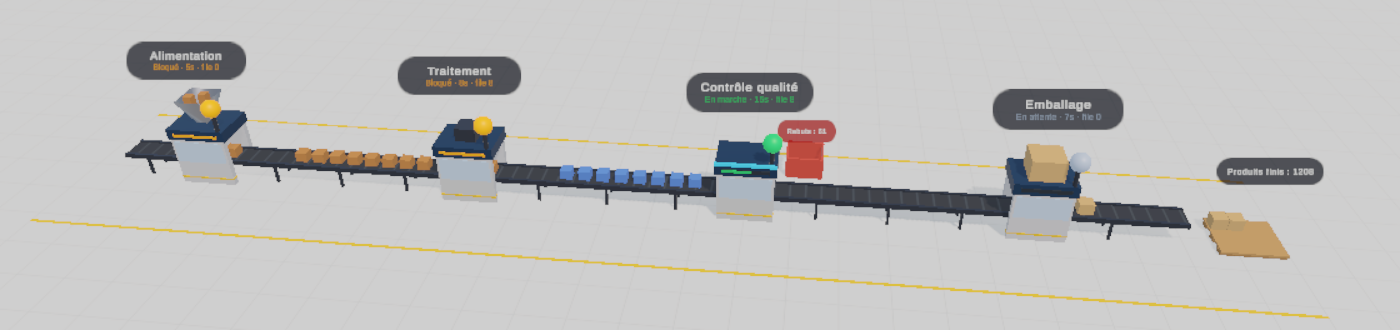
\includegraphics[width=\textwidth]{images/screenshots/vue_globale.png}
\caption{Vue d'ensemble de la scène Unity (build WebGL, ligne initiale). Les produits s'accumulent devant le contrôle qualité, le traitement et l'alimentation sont bloqués en amont~; le bac rouge reçoit les rebuts, la palette les produits finis.}
\label{fig:vue_globale}
\end{figure}

\subsection{Fluidité}

Les produits ne sont pas déplacés par un calcul propre à la scène~: le client conserve un tampon des derniers états reçus (10~Hz) et affiche la ligne \textbf{avec un léger retard de 0{,}15~s}, ce qui permet d'interpoler la position de chaque produit entre deux états consécutifs à la cadence de l'écran. Le mouvement reste ainsi continu même si un message arrive en retard. Les produits sont recyclés dans un \textit{pool} (aucune allocation par image), les machines et le décor n'ont pas de collider inutile et le matériel du convoyeur est animé par un décalage de texture. Dans le build WebGL, le premier chargement prend quelques secondes (environ 12~Mo compressés).

\subsection{Difficultés rencontrées}

Deux points techniques méritent d'être signalés. D'abord, dans un build WebGL réduit au minimum, les colliders de capsule, sphère et maillage sont supprimés~: créer une primitive par \code{GameObject.CreatePrimitive} à l'exécution produisait des erreurs dans la console du navigateur. Les formes créées pendant l'exécution partent donc de maillages partagés, sans collider~; seule la zone cliquable des quatre machines garde un \code{BoxCollider}. Ensuite, un brouillard trop dense voilait la scène dans une fenêtre étroite~: il est désormais calculé à partir de la distance de la caméra.

\begin{figure}[H]
\centering
\begin{subfigure}[t]{0.49\textwidth}
  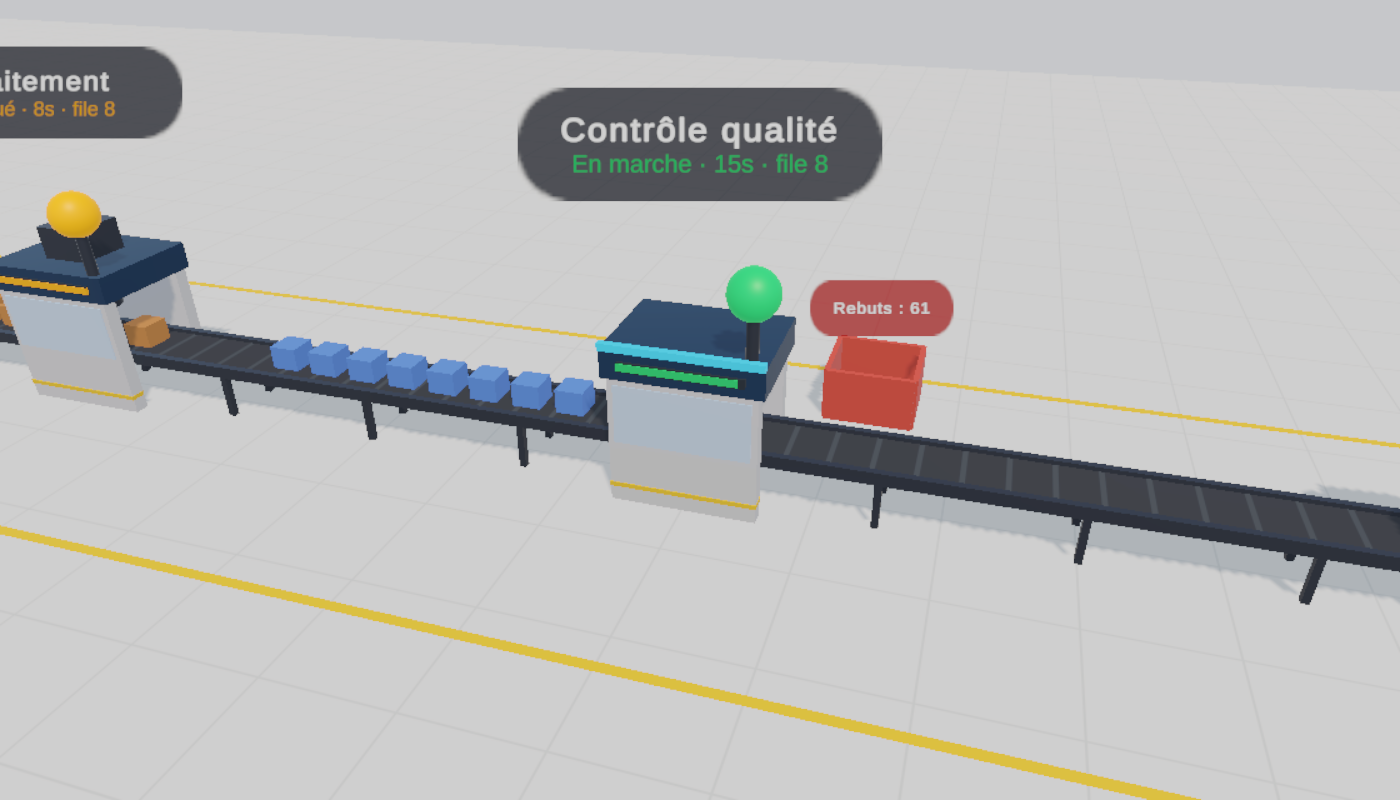
\includegraphics[width=\textwidth]{images/screenshots/zoom_controle.png}
  \caption{Zoom sur une machine~: étiquette d'état, voyant et barre de progression.}
\end{subfigure}\hfill
\begin{subfigure}[t]{0.49\textwidth}
  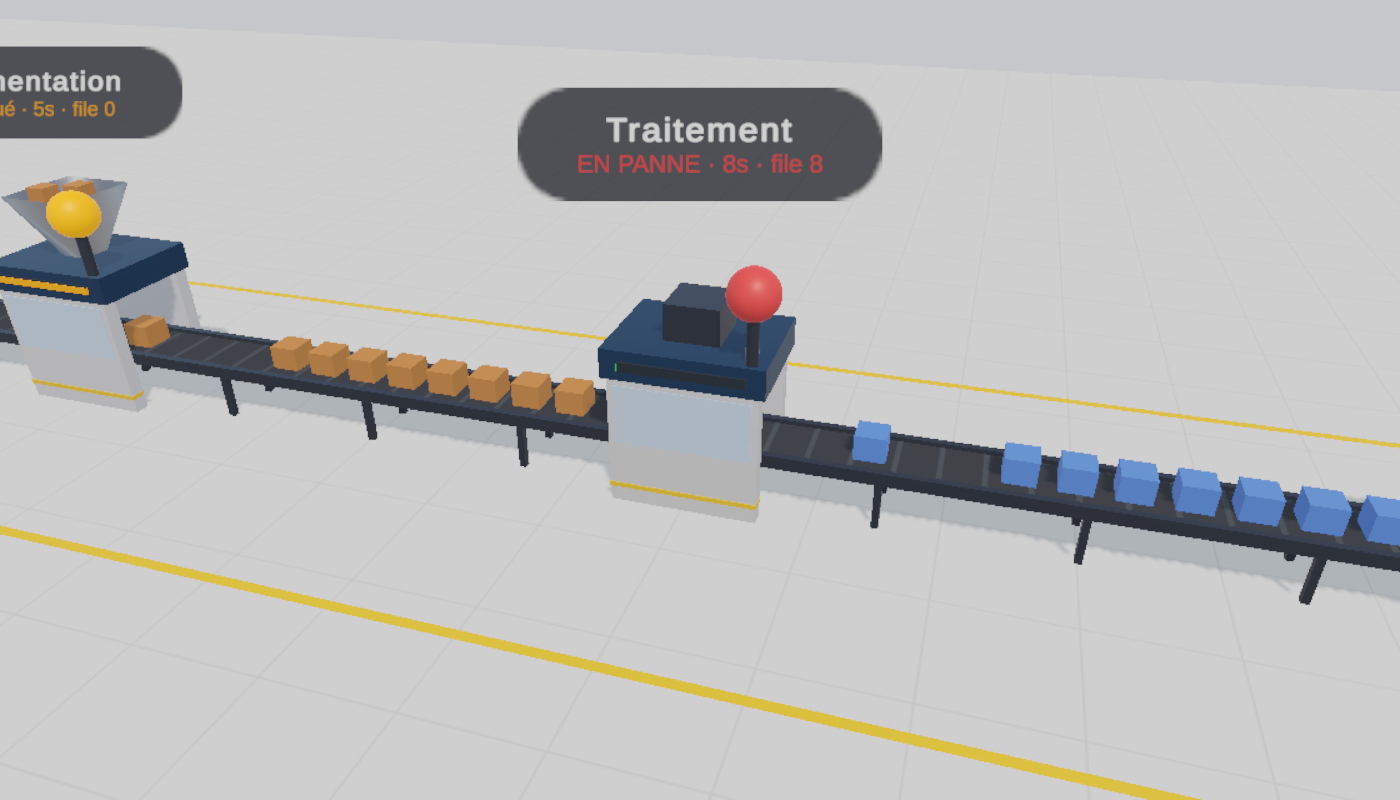
\includegraphics[width=\textwidth]{images/screenshots/panne_traitement.png}
  \caption{Panne provoquée sur le traitement~: voyant rouge, file amont pleine.}
\end{subfigure}
\caption{États visuels dans la scène Unity.}
\label{fig:etats_3d}
\end{figure}

\section{Le tableau de bord (\code{app.js})}

Le panneau latéral comporte trois onglets. \textbf{Supervision} affiche les \ac{KPI}, le tableau des postes, la courbe de débit des trois dernières minutes avec le débit théorique, les réglages du scénario, la fiche de la machine sélectionnée (\ac{MTBF}, \ac{MTTR}, disponibilité) et le journal. \textbf{Historique} relit la base SQLite par l'\ac{API} \ac{REST}. \textbf{Aide} résume la prise en main.

\begin{figure}[H]
\centering
\begin{subfigure}[t]{0.32\textwidth}
  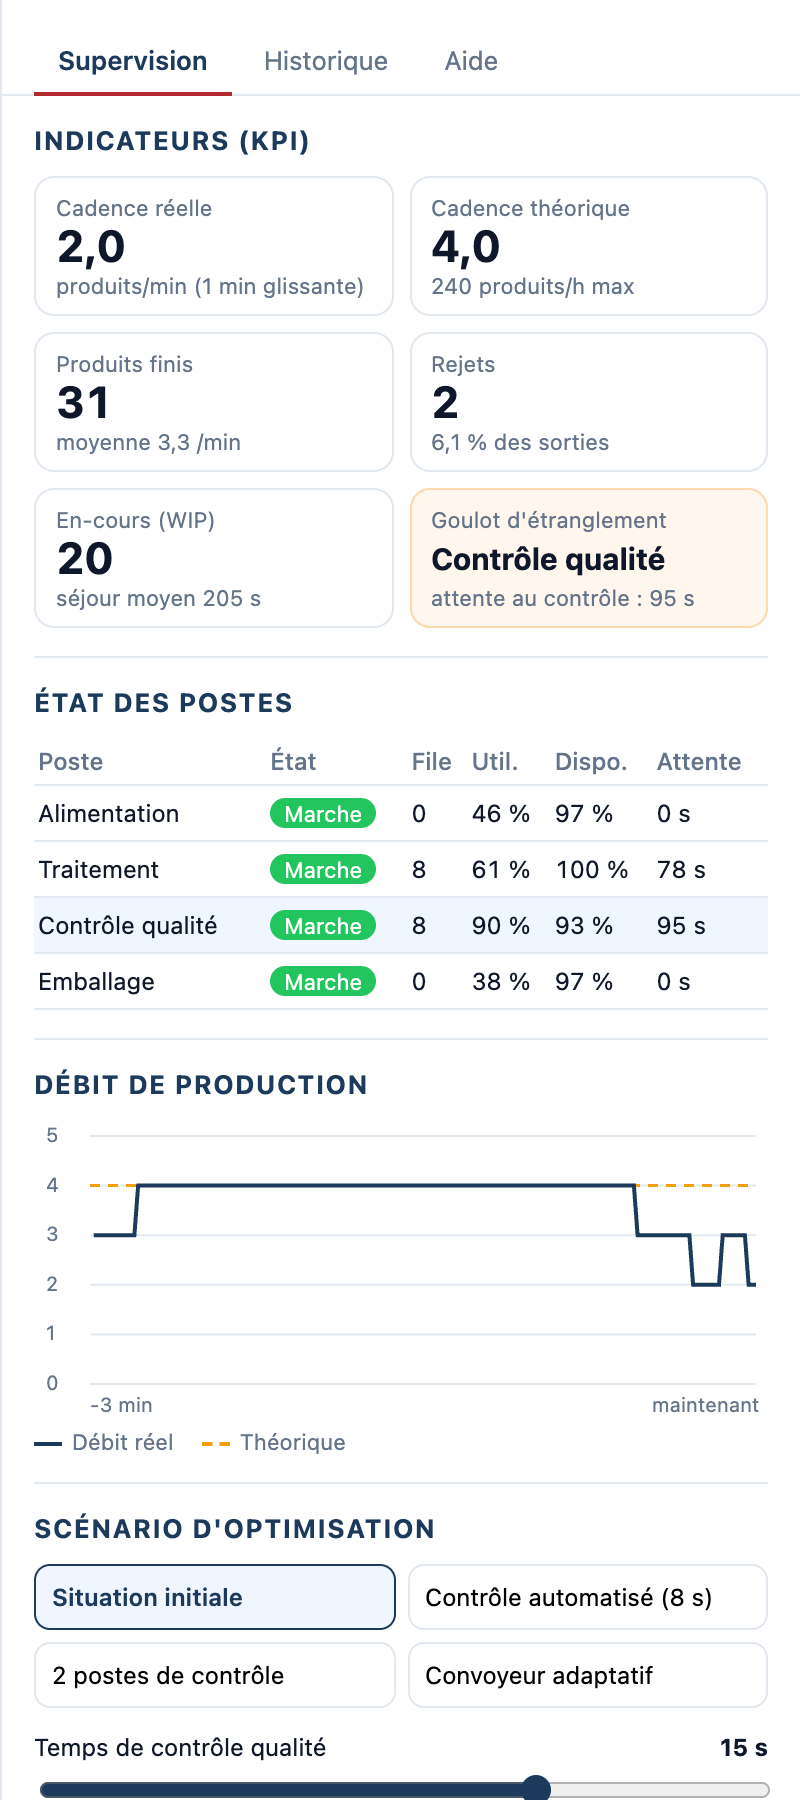
\includegraphics[width=\textwidth]{images/screenshots/dashboard_kpi.png}
  \caption{Supervision.}
\end{subfigure}\hfill
\begin{subfigure}[t]{0.32\textwidth}
  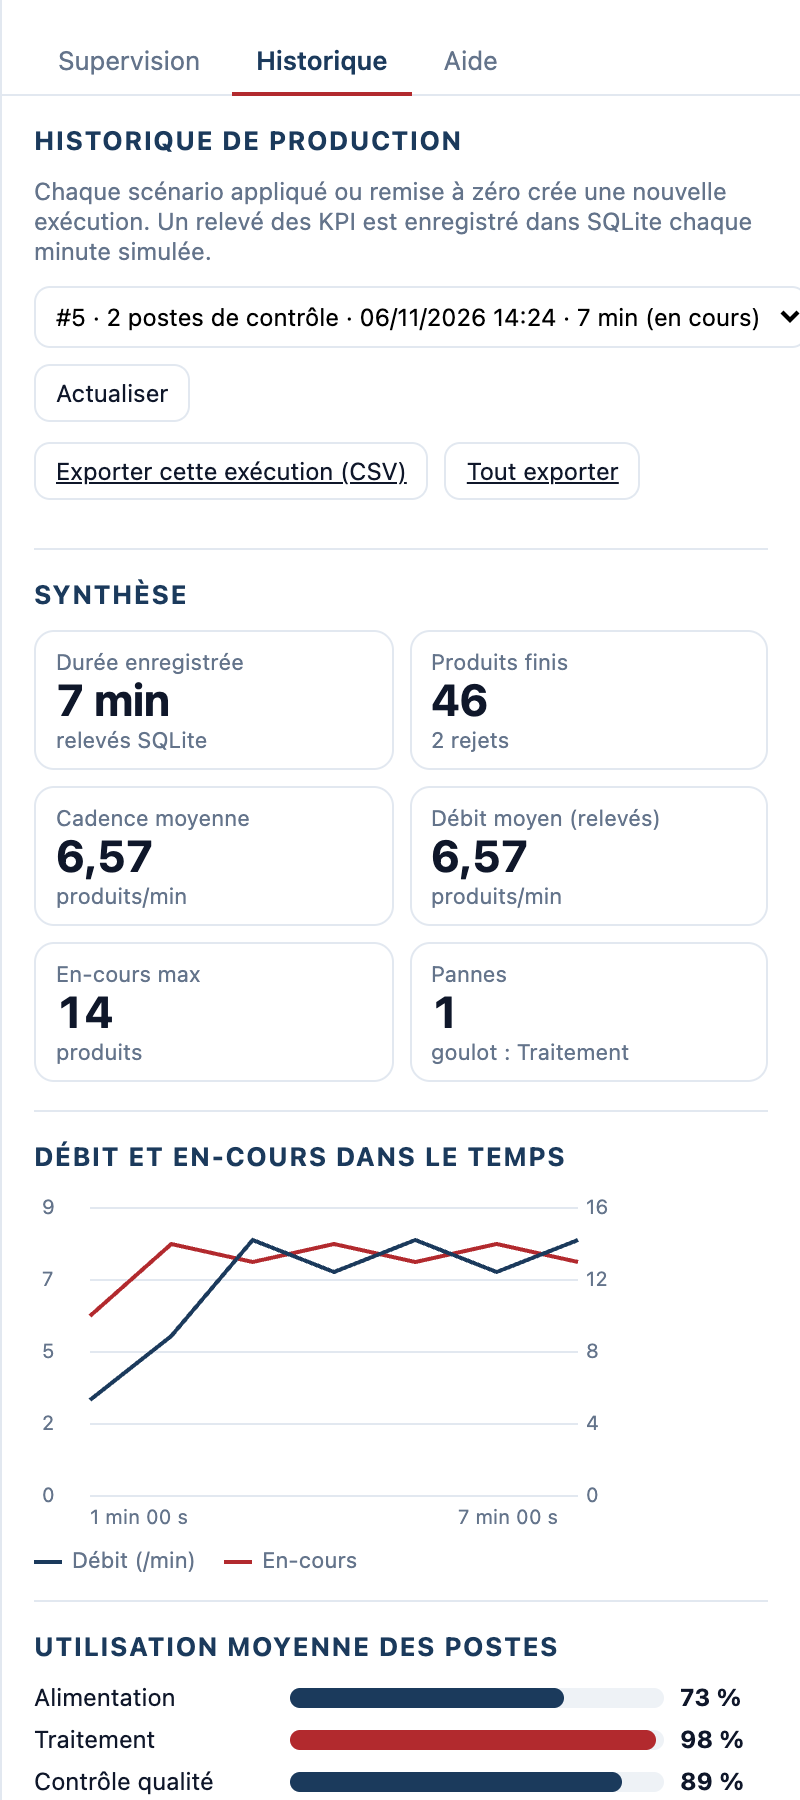
\includegraphics[width=\textwidth]{images/screenshots/historique.png}
  \caption{Historique (SQLite).}
\end{subfigure}\hfill
\begin{subfigure}[t]{0.32\textwidth}
  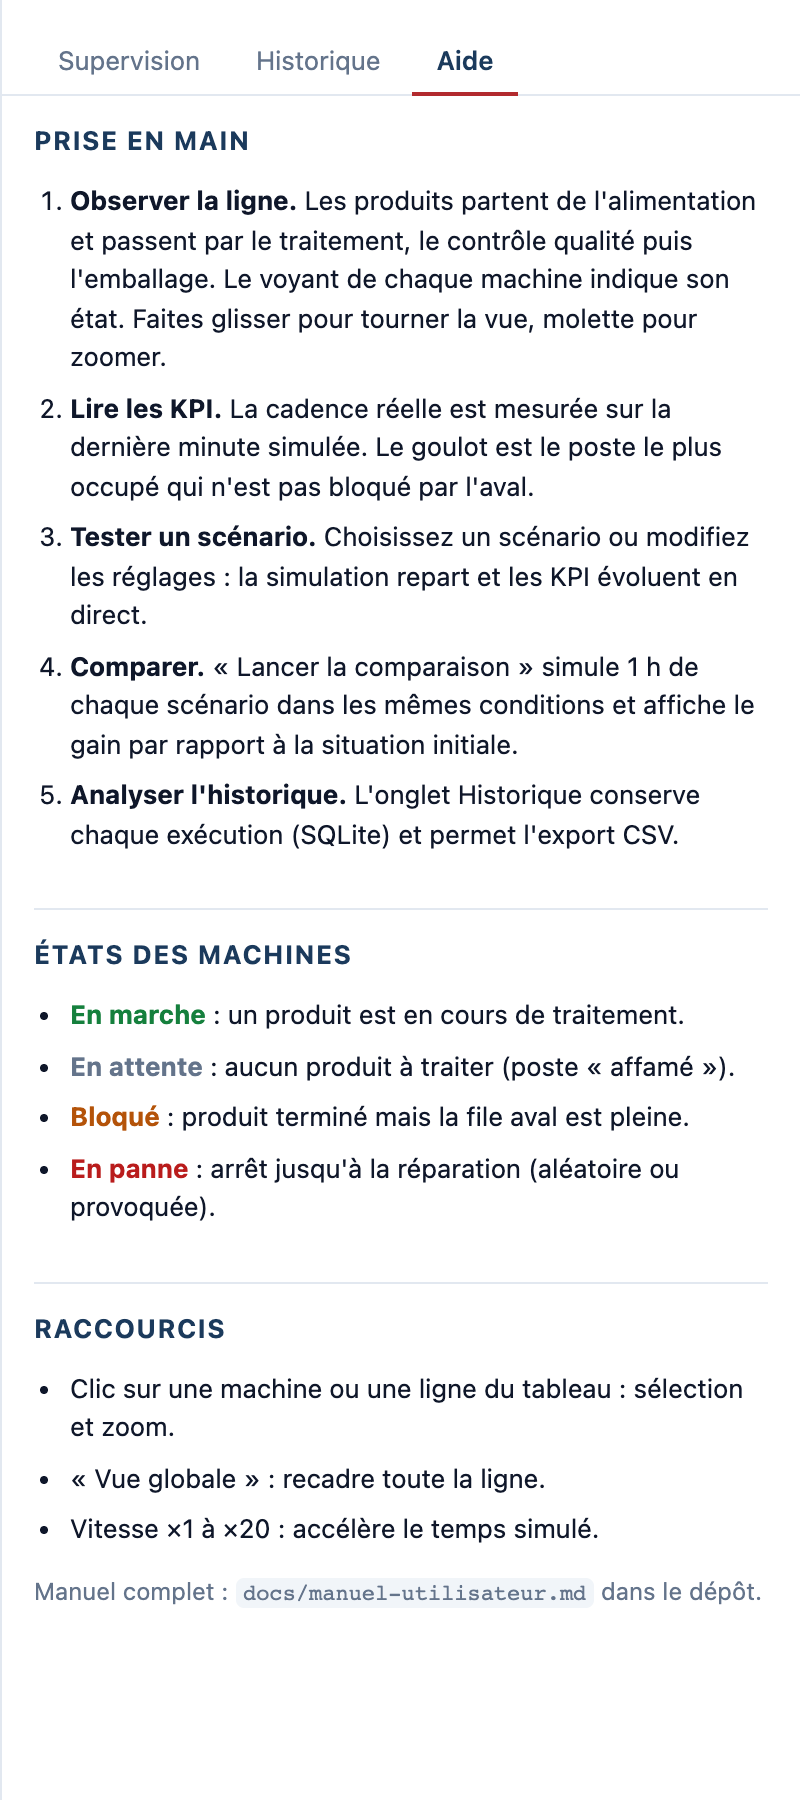
\includegraphics[width=\textwidth]{images/screenshots/aide.png}
  \caption{Aide.}
\end{subfigure}
\caption{Les trois onglets du tableau de bord.}
\label{fig:dashboard}
\end{figure}

\section{Validation du modèle}

Mohamed \textsc{Hamdouch} étant responsable de la validation, le modèle est vérifié par \textbf{23 tests automatisés} (pytest), exécutés en moins d'une minute. Ils ne vérifient pas que le code \enquote{tourne}, mais que la simulation respecte des propriétés connues d'une ligne de production~:

\begin{table}[H]
\centering
\caption{Propriétés vérifiées par les tests automatisés.}
\label{tab:tests}
\begin{tabularx}{\textwidth}{@{}X l@{}}
\toprule
\textbf{Propriété vérifiée} & \textbf{Résultat} \\
\midrule
Débit de régime (sans pannes ni rejets) égal au débit théorique à 5~\% près~: 4,0 / 7,5 / 7,5 produits/min & 3/3 \\
Conservation~: produits créés = finis + rejetés + en-cours, pour chaque scénario & 4/4 \\
Aucune file ne dépasse sa capacité (8, ou 3 en mode adaptatif) & 4/4 \\
Utilisation et disponibilité comprises entre 0 et 1 & 1/1 \\
Les pannes réduisent la disponibilité et la production~; une panne provoquée arrête le poste & 2/2 \\
Taux de rejet observé proche de 5~\% sur 4~h simulées & 1/1 \\
Le goulot est identifié au contrôle, puis déplacé au traitement après optimisation & 1/1 \\
Le convoyeur adaptatif réduit l'en-cours sans perte de débit & 1/1 \\
Comparaison reproductible à graine identique~; ajout et retrait de machines sans perte de produit & 2/2 \\
Historique~: relevés, événements, export \ac{CSV}~; \ac{API} \ac{WS} et \ac{REST} & 4/4 \\
\midrule
\textbf{Total} & \textbf{23/23} \\
\bottomrule
\end{tabularx}
\end{table}

Un contrôle supplémentaire est fourni par la \textbf{loi de Little}~\cite{little1961}, $L = \lambda W$~: l'en-cours moyen doit égaler le débit d'entrée multiplié par le temps de séjour moyen. Sur la ligne initiale avec pannes, $\lambda = (218 + 12)/3600$~produits/s et $W = 286$~s donnent $L \approx 18{,}3$, pour un en-cours moyen mesuré de 19{,}0. L'écart de 4~\% s'explique par les produits encore en ligne en fin de simulation, dont le séjour n'est pas compté dans $W$.

% ============================================================================
% Chapitre 5 --- Scénario d'optimisation
% ============================================================================
\chapter{Scénario d'optimisation}
\label{chap:optimisation}

\begin{callout}
\textbf{Objectif~:} réduire le goulot d'étranglement au poste de contrôle qualité afin d'augmenter le débit global de la ligne de production.
\end{callout}

\section{Problème identifié}

Avec les paramètres initiaux (tableau~\ref{tab:parametres}), le contrôle qualité est le poste le plus lent~: 15~s par produit contre 8~s au traitement. Le jumeau numérique rend le phénomène visible sans calcul (figure~\ref{fig:vue_globale})~: au bout de quelques minutes, la file devant le contrôle atteint sa capacité de 8 produits, le traitement se bloque faute de place, puis l'alimentation à son tour. Le tableau de bord confirme le diagnostic~: le contrôle qualité est utilisé à 96~\% du temps, contre 53~\% pour le traitement et 35~\% pour l'alimentation, et un produit y attend en moyenne près de deux minutes.

\section{Solutions testées}

\begin{enumerate}
  \item \textbf{Contrôle automatisé}~: le temps de contrôle passe de 15 à 8~s grâce à une inspection automatisée. Cadence théorique~: $60/8 = 7{,}5$~produits/min, le traitement (8~s) devenant le nouveau poste limitant.
  \item \textbf{Deuxième poste de contrôle}~: deux machines de 15~s en parallèle, soit un temps effectif de 7{,}5~s. Cadence théorique~: 7{,}5~produits/min, limitée là aussi par le traitement.
  \item \textbf{Convoyeur adaptatif}~: le convoyeur ralentit devant une file chargée et la file maximale passe de 8 à 3 produits. Le débit théorique ne change pas (4~produits/min)~: cette solution vise l'accumulation, pas la cadence.
\end{enumerate}

\section{Protocole de comparaison}

Comparer deux scénarios en regardant l'animation n'est pas fiable~: une panne tombée au mauvais moment dans l'un des deux suffit à inverser la conclusion. Chaque scénario est donc simulé \textbf{pendant une heure}, sans affichage, avec la \textbf{même graine aléatoire} et les mêmes paramètres de fiabilité, de transfert et de rejet. Le bouton \enquote{Lancer la comparaison} du tableau de bord exécute exactement ce protocole (fonction \code{compare\_presets})~; les chiffres ci-dessous en sont la sortie brute, conservée dans \code{docs/\allowbreak rapport/\allowbreak data/\allowbreak resultats.json}.

\section{Résultats}

\begin{table}[H]
\centering
\caption{Comparaison avant / après sur 1~h simulée, pannes activées (graine 7).}
\label{tab:resultats}
\small
\begin{tabularx}{\textwidth}{@{}X cccc@{}}
\toprule
\textbf{Indicateur} & \textbf{Initiale} & \textbf{Contrôle 8~s} & \textbf{2 contrôles} & \textbf{Adaptatif} \\
\midrule
Produits finis / h & 218 & \textbf{390} (+79~\%) & 389 (+78~\%) & 218 (0~\%) \\
Cadence moyenne (/min) & 3,63 & \textbf{6,50} & 6,48 & 3,63 \\
Cadence théorique (/min) & 4,0 & 7,5 & 7,5 & 4,0 \\
Attente au contrôle (s) & 115 & \textbf{9} ($-$92~\%) & 16 ($-$86~\%) & 41 ($-$65~\%) \\
En-cours moyen (produits) & 19,0 & 13,4 ($-$30~\%) & 14,9 ($-$22~\%) & \textbf{9,4} ($-$51~\%) \\
Temps de séjour moyen (s) & 286 & \textbf{113} ($-$60~\%) & 129 ($-$55~\%) & 145 ($-$49~\%) \\
Rejets & 12 & 23 & 23 & 12 \\
Pannes / arrêts cumulés (s) & 25 / 589 & 28 / 635 & 29 / 712 & 25 / 589 \\
Goulot observé & Contrôle & Traitement & Traitement & Contrôle \\
\bottomrule
\end{tabularx}
\end{table}

\begin{figure}[H]
\centering
\begin{tikzpicture}
\begin{axis}[
  ybar, bar width=16pt, width=0.95\textwidth, height=6.2cm,
  ylabel={Produits finis par heure}, ymin=0, ymax=470,
  symbolic x coords={Initiale, Contrôle 8 s, 2 contrôles, Adaptatif},
  xtick=data, nodes near coords, nodes near coords style={font=\footnotesize},
  enlarge x limits=0.18, legend style={at={(0.5,1.03)}, anchor=south, legend columns=2, font=\footnotesize, draw=none},
  ymajorgrids, grid style={gray!20}, axis line style={gray!60}, tick label style={font=\footnotesize}
]
\addplot[fill=ensambleu, draw=ensambleu] coordinates {(Initiale,218) (Contrôle 8 s,390) (2 contrôles,389) (Adaptatif,218)};
\addplot[fill=ensambleu!35, draw=ensambleu!35] coordinates {(Initiale,226) (Contrôle 8 s,422) (2 contrôles,421) (Adaptatif,226)};
\legend{Avec pannes, Sans pannes}
\end{axis}
\end{tikzpicture}
\caption{Production horaire par scénario, avec et sans pannes.}
\label{fig:production}
\end{figure}

\begin{figure}[H]
\centering
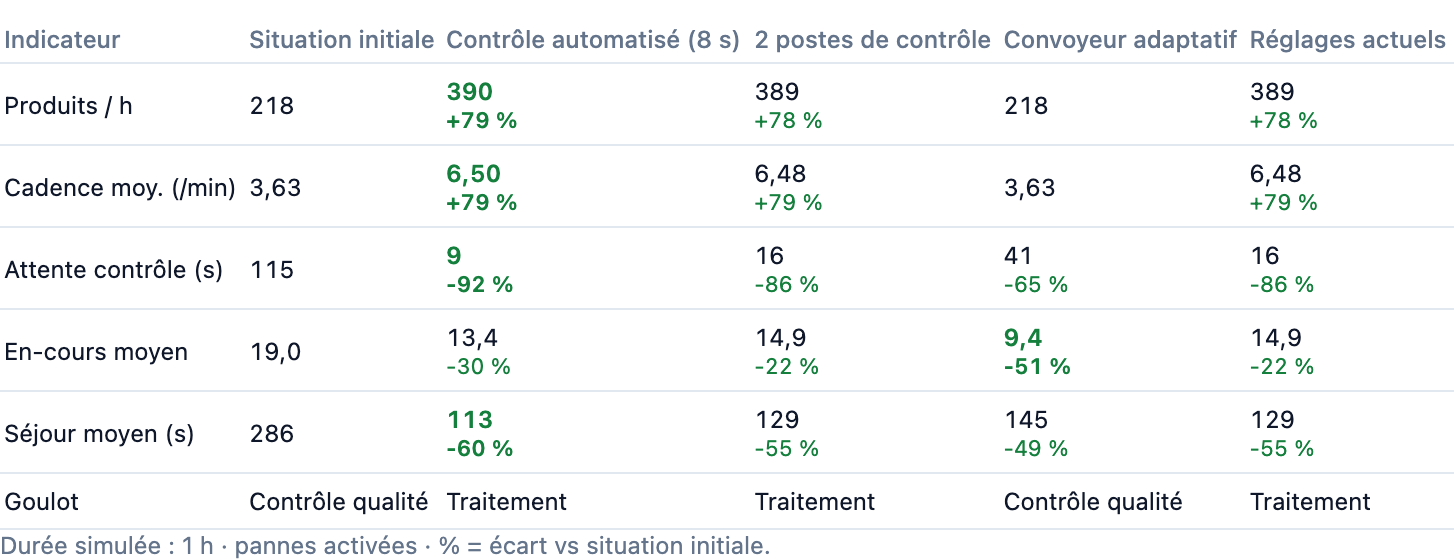
\includegraphics[width=\textwidth]{images/screenshots/comparaison.png}
\caption{Le même tableau dans l'interface (bouton \enquote{Lancer la comparaison})~; la colonne \enquote{Réglages actuels} reprend la configuration en cours.}
\label{fig:cmp_ui}
\end{figure}

\section{Analyse}

\paragraph{Le goulot se déplace.} Les deux premières solutions augmentent la production d'environ 79~\%, et le goulot passe du contrôle au traitement, comme prévu par le calcul théorique~: le traitement est désormais utilisé à 94~\% du temps. Toute amélioration supplémentaire devra donc porter sur le traitement. C'est le principe central de la théorie des contraintes~: optimiser un poste qui n'est pas le goulot ne sert à rien, et optimiser le goulot en fait apparaître un autre.

\paragraph{Contrôle automatisé ou deuxième poste~?} À débit égal, le contrôle automatisé est légèrement meilleur sur l'attente (9~s contre 16~s) et sur le temps de séjour, parce qu'un produit traverse le contrôle en 8~s au lieu de 15. Sur une ligne réelle, le deuxième poste apporterait en plus une redondance~: si l'une des deux machines tombe en panne, l'autre continue à 4~produits/min. Notre modèle ne capture pas cet avantage, car il traite la panne au niveau du poste entier (les deux machines s'arrêtent ensemble)~; c'est l'une des améliorations listées en perspective. Le choix entre les deux dépend donc d'informations que la simulation ne contient pas~: coût de l'automatisation, coût d'un poste et d'un opérateur supplémentaires, criticité des arrêts.

\paragraph{Le convoyeur adaptatif ne produit pas plus.} Il réduit l'en-cours de moitié et l'attente des deux tiers, sans perte de débit~; mais il ne déplace pas le goulot. Il a du sens en complément d'une des deux premières solutions (moins de stock entre postes, moins de produits immobilisés), pas à leur place.

\paragraph{Écart entre théorie et simulation.} L'énoncé estimait 240 produits/h avant et 450 après. La simulation donne 218 et 390. Sans pannes, la ligne initiale produit 226 produits finis \textbf{et} 12 rejetés, soit 238 produits sortis du contrôle~: l'écart restant avec 240 correspond au temps de démarrage (le premier produit n'atteint le contrôle qu'après 17~s, et le premier produit fini ne sort qu'après 41~s). Les pannes coûtent ensuite environ 4~\% de production sur la ligne initiale et 8~\% après optimisation~: une ligne plus rapide perd davantage de produits pour une même minute d'arrêt. Enfin, l'objectif de 450 produits/h n'est pas atteint, même sans pannes (422 finis + 24 rejets = 446 sorties)~: les 5~\% de rejets et le démarrage suffisent à l'expliquer. Le jumeau numérique a donc corrigé l'estimation initiale à la baisse de 13~\%, ce qui est précisément son rôle avant un investissement réel.

\begin{warn}
\textbf{Limite de la comparaison.} La graine aléatoire est identique pour tous les scénarios, mais les tirages divergent dès que la séquence d'événements diffère (un produit de plus contrôlé consomme un tirage de rejet de plus). Les pannes ne tombent donc pas exactement aux mêmes instants d'un scénario à l'autre. Pour des conclusions plus solides, il faudrait répéter la comparaison sur plusieurs graines et présenter des intervalles de confiance~; avec des écarts de l'ordre de 80~\%, la conclusion principale ne fait cependant pas de doute.
\end{warn}

\section{Démonstration dans le jumeau numérique}

\begin{enumerate}
  \item \textbf{Avant optimisation}~: lancer la situation initiale à vitesse $\times$10~; observer l'accumulation devant le contrôle, le blocage de l'amont et l'attente affichée (environ deux minutes).
  \item \textbf{Incident}~: provoquer une panne sur le traitement~; le voyant passe au rouge et la cadence chute.
  \item \textbf{Après optimisation}~: appliquer le contrôle automatisé à 8~s ou le deuxième poste~; la file se résorbe en quelques minutes et le goulot affiché passe au traitement.
  \item \textbf{Comparaison}~: lancer la comparaison, puis consulter et exporter les deux exécutions dans l'onglet Historique.
\end{enumerate}

% ============================================================================
% Chapitre 6 --- Aspects organisationnels et humains
% ============================================================================
\chapter{Aspects organisationnels et humains}
\label{chap:organisation}

Un jumeau numérique ne crée de la valeur que s'il est utilisé par les personnes qui pilotent la ligne. Ce chapitre répond à la troisième partie du cahier des charges, en se plaçant dans l'hypothèse d'un déploiement du jumeau dans un atelier réel.

\section{Formation des opérateurs}

\begin{table}[H]
\centering
\caption{Parcours de formation proposé.}
\label{tab:formation}
\begin{tabularx}{\textwidth}{@{}p{2.6cm} p{1.5cm} X p{3.2cm}@{}}
\toprule
\textbf{Public} & \textbf{Durée} & \textbf{Contenu} & \textbf{Support} \\
\midrule
Opérateurs de ligne & 1~h & Lire la scène 3D (voyants, files, couleurs des produits), lire les \ac{KPI}, signaler un écart entre le jumeau et la ligne & Onglet Aide, démonstration guidée \\
Chefs d'équipe & 2~h & Piloter un scénario, provoquer une panne en formation, lire l'historique, exporter les données & Manuel utilisateur, exercices \\
Méthodes et maintenance & 0,5~journée & Notion de goulot, comparaison de scénarios, interprétation des écarts théorie/simulation, \ac{MTBF} et \ac{MTTR} & Rapport, données \ac{CSV} \\
Équipe informatique & 0,5~journée & Architecture, protocole \ac{WS}, base SQLite, ajout d'un poste, tests & README, code et tests \\
\bottomrule
\end{tabularx}
\end{table}

Le jumeau sert lui-même d'outil de formation~: on peut provoquer une panne ou saturer un poste \textbf{sans aucun risque} pour la production, et montrer en quelques minutes simulées des phénomènes qui prendraient des heures à observer sur la ligne réelle.

\section{Adaptation des processus de travail}

\begin{itemize}
  \item \textbf{Décision d'amélioration}~: toute modification de la ligne (temps de cycle, ajout d'un poste, nouvelle règle de convoyage) est d'abord simulée et comparée dans les mêmes conditions que la situation actuelle~; la décision s'appuie sur le tableau de comparaison exporté.
  \item \textbf{Réunions de production}~: la revue quotidienne s'appuie sur l'historique (débit par heure, pannes, goulot observé) plutôt que sur des relevés manuels.
  \item \textbf{Maintenance}~: les \ac{MTBF} et \ac{MTTR} observés par poste orientent la maintenance préventive vers les postes dont la panne coûte le plus de production, c'est-à-dire en priorité le goulot.
  \item \textbf{Écart jumeau/réalité}~: un processus de recalage est nécessaire. Lorsque la ligne réelle s'écarte durablement de la simulation, les paramètres du modèle (temps de cycle, \ac{MTBF}, taux de rejet) sont mis à jour à partir des données mesurées.
\end{itemize}

\section{Gestion du changement}

L'introduction d'un outil de supervision peut être perçue comme un outil de surveillance individuelle. Quatre mesures limitent ce risque~:

\begin{enumerate}
  \item \textbf{Associer les opérateurs dès la conception}~: ils connaissent les micro-arrêts et les contournements que les données ne montrent pas, et leur retour améliore la fidélité du modèle.
  \item \textbf{Mesurer la ligne, pas les personnes}~: les \ac{KPI} affichés portent sur les postes et le flux, jamais sur un individu.
  \item \textbf{Déployer progressivement}~: d'abord en salle de formation, puis en supervision passive à côté de la ligne, avant de l'utiliser pour décider d'investissements.
  \item \textbf{Montrer un premier gain concret}~: le scénario du contrôle qualité, qui ne demande qu'une modification de poste pour un gain de près de 80~\%, est un bon premier cas d'usage à présenter.
\end{enumerate}

\section{Organisation de l'équipe projet}

Le projet a été mené par une équipe de six, organisée selon la répartition du tableau~\ref{tab:roles}. Le travail suit les sept phases du plan de travail (annexe~\ref{ann:planning})~: analyse du besoin, modélisation \ac{3D}, simulation, backend, tableau de bord, optimisation et validation, rédaction. Le code est versionné dans un dépôt Git privé, et chaque responsabilité correspond à un fichier principal, ce qui limite les conflits entre membres. Les tests automatisés jouent le rôle de garde-fou commun~: une modification qui casse une propriété du modèle est détectée avant d'être intégrée.

% ============================================================================
% Chapitre 7 --- Conclusion et perspectives
% ============================================================================
\chapter{Conclusion et perspectives}
\label{chap:conclusion}

\section{Bilan des livrables}

\begin{table}[H]
\centering
\caption{Bilan des livrables du cahier des charges.}
\label{tab:bilan}
\begin{tabularx}{\textwidth}{@{}X X c@{}}
\toprule
\textbf{Livrable} & \textbf{Réalisation} & \textbf{Statut} \\
\midrule
Modèle de simulation du système physique & \code{sim.py}~: 4 postes, files, blocages, pannes, rejets, \ac{KPI} & Livré \\
Interface synchronisée avec des données simulées & Scène 3D Unity (WebGL) et tableau de bord sur un flux \ac{WS} unique à 10~Hz & Livré \\
Scénario d'optimisation testé et documenté & 3 solutions comparées sur 1~h simulée avec la scène Unity, chapitre~\ref{chap:optimisation} & Livré \\
Historique et statistiques de production & SQLite, onglet Historique, export \ac{CSV} & Livré \\
Validation du modèle & 23 tests automatisés, contrôle par la loi de Little & Livré \\
Rapport, présentation, manuel utilisateur & Ce document, support de soutenance, \code{docs/manuel-utilisateur.md} & Livré \\
\bottomrule
\end{tabularx}
\end{table}

Le résultat principal est le suivant~: sur une heure simulée avec pannes, réduire le temps de contrôle de 15 à 8~s, ou doubler le poste de contrôle, fait passer la production de 218 à environ 393 produits finis, soit +80~\%, et déplace le goulot vers le traitement. Ces valeurs ont été mesurées avec la scène Unity connectée au backend et recoupent la simulation hors ligne à 1{,}3~\% près. Le jumeau a aussi corrigé l'estimation théorique de départ (450~produits/h) en tenant compte des rejets, des transferts et des pannes.

\section{Limites assumées}

\begin{itemize}
  \item \textbf{Les données sont entièrement simulées.} La ligne \enquote{physique} est elle-même un modèle~; les temps de cycle, \ac{MTBF} et taux de rejet sont des hypothèses pédagogiques. Les conclusions valent pour ce modèle, pas pour une ligne réelle tant que ses paramètres n'ont pas été mesurés.
  \item \textbf{Pas de connexion à des équipements réels.} Il n'y a ni automate, ni capteur, ni protocole industriel~: le jumeau n'est pas encore relié à un système physique au sens strict de Kritzinger et al.~\cite{kritzinger2018}.
  \item \textbf{Pannes au niveau du poste.} Quand un poste a deux machines, une panne les arrête toutes les deux~; la redondance d'un poste doublé n'est donc pas modélisée.
  \item \textbf{Une seule graine par comparaison.} Les résultats ne sont pas accompagnés d'intervalles de confiance (chapitre~\ref{chap:optimisation}).
  \item \textbf{Fluidité non chiffrée.} Le nombre d'images par seconde du build WebGL dépend du poste~; il doit être relevé sur la machine de démonstration.
  \item \textbf{Sécurité minimale.} L'application est prévue pour un usage local~: pas d'authentification ni de chiffrement.
\end{itemize}

\section{Perspectives}

\begin{enumerate}
  \item \textbf{Connecter une source réelle}~: remplacer \code{sim.py} par un adaptateur \ac{OPC} ou MQTT qui lit l'état d'automates, en conservant le même format de message~; la \ac{3D} et le tableau de bord n'auraient pas à changer.
  \item \textbf{Recalage automatique}~: estimer les temps de cycle et les \ac{MTBF} à partir de l'historique réel et mettre à jour le modèle.
  \item \textbf{Maintenance prédictive}~: exploiter l'historique des pannes pour prévoir les arrêts et planifier la maintenance du goulot.
  \item \textbf{Optimisation automatique}~: explorer automatiquement l'espace des réglages (temps, nombre de machines, tailles de files) pour trouver le meilleur compromis débit/en-cours, sur plusieurs graines.
  \item \textbf{Indicateurs industriels}~: ajouter le \ac{TRS} (disponibilité $\times$ performance $\times$ qualité) par poste.
  \item \textbf{Déploiement}~: authentification, rôles (consultation ou pilotage), chiffrement, hébergement sur le réseau de l'atelier.
\end{enumerate}

\section{Compétences mobilisées}

Ce projet nous a fait traverser toute la chaîne d'un jumeau numérique~: modélisation d'un système de production et de ses phénomènes (goulot, blocage, fiabilité), programmation d'une simulation, communication temps réel entre un serveur et des clients, rendu \ac{3D} avec Unity exporté en WebGL, conception d'indicateurs et d'une interface de supervision, validation par des tests et par des lois connues, et travail en équipe autour d'un protocole commun. Il illustre ce qui distingue un jumeau numérique d'une simple animation~: chaque chiffre affiché peut être relié au modèle, vérifié et reproduit.


\clearpage
\phantomsection
\addcontentsline{toc}{chapter}{Bibliographie et webographie}
\renewcommand{\bibname}{Bibliographie et webographie}
\bibliographystyle{unsrt}
\bibliography{references}

\appendix
\chapter{Planning et ressources}
\label{ann:planning}

\section{Planning par phases}

\begin{table}[H]
\centering
\caption{Phases du projet et responsables (planning prévisionnel en semaines).}
\label{tab:planning}
\small
\begin{tabularx}{\textwidth}{@{}c X l *{7}{c}@{}}
\toprule
\textbf{Ph.} & \textbf{Travail} & \textbf{Responsable(s)} & \textbf{S1} & \textbf{S2} & \textbf{S3} & \textbf{S4} & \textbf{S5} & \textbf{S6} & \textbf{S7} \\
\midrule
1 & Analyse du besoin, conception, protocole & Tous & \cellcolor{ensambleu} & & & & & & \\
2 & Modélisation et animation 3D & Issami, Ezbakhe & & \cellcolor{ensambleu} & \cellcolor{ensambleu} & & & & \\
3 & Simulation industrielle & Benzahra & & \cellcolor{ensambleu} & \cellcolor{ensambleu} & & & & \\
4 & Backend, communication, stockage & Hsain & & & \cellcolor{ensambleu} & \cellcolor{ensambleu} & & & \\
5 & Dashboard et indicateurs & Kichchou & & & & \cellcolor{ensambleu} & \cellcolor{ensambleu} & & \\
6 & Optimisation, tests, validation & Hamdouch & & & & & \cellcolor{ensambleu} & \cellcolor{ensambleu} & \\
7 & Rapport et présentation & Tous & & & & & & \cellcolor{ensambleu} & \cellcolor{ensambleu} \\
\bottomrule
\end{tabularx}
\end{table}

\section{Ressources}

\begin{table}[H]
\centering
\caption{Ressources nécessaires.}
\label{tab:ressources}
\begin{tabularx}{\textwidth}{@{}l X r@{}}
\toprule
\textbf{Type} & \textbf{Ressource} & \textbf{Coût} \\
\midrule
Matériel & Ordinateurs personnels de l'équipe, navigateur récent compatible WebGL & 0 \\
Logiciels & Python 3.12, FastAPI, Uvicorn, pytest, SQLite, Three.js (open source) & 0 \\
Collaboration & Dépôt Git privé (GitHub), éditeurs de code & 0 \\
Documentation & \LaTeX{} (tectonic) pour le rapport, HTML pour la présentation & 0 \\
\midrule
\textbf{Total} & & \textbf{0~MAD} \\
\bottomrule
\end{tabularx}
\end{table}

\section{Critères d'évaluation}

\begin{table}[H]
\centering
\caption{Critères du cahier des charges et éléments de preuve.}
\label{tab:criteres}
\begin{tabularx}{\textwidth}{@{}l X@{}}
\toprule
\textbf{Critère} & \textbf{Élément de preuve} \\
\midrule
Atteinte des objectifs fixés & Les trois livrables sont réalisés (tableau~\ref{tab:bilan}) \\
Respect des délais et du budget & Planning par phases, aucun coût (tableau~\ref{tab:ressources}) \\
Qualité de la réalisation technique & 23 tests automatisés, loi de Little vérifiée, architecture découplée \\
Facilité d'utilisation pour les opérateurs & Scène 3D, voyants d'état, onglet Aide, manuel utilisateur \\
\bottomrule
\end{tabularx}
\end{table}

\chapter{Résultats des tests automatisés}
\label{ann:tests}

Sortie de \code{python -m pytest -rA} sur le dépôt (23 tests, tous réussis).

\begin{lstlisting}[language={}, numbers=none, basicstyle=\ttfamily\scriptsize]
tests/test_api.py::test_websocket_etat_et_commandes                         PASSED
tests/test_api.py::test_api_historique_et_export                            PASSED
tests/test_sim.py::test_debit_regime_egal_au_debit_theorique[initial-4.0]   PASSED
tests/test_sim.py::test_debit_regime_egal_au_debit_theorique[controle_auto-7.5]   PASSED
tests/test_sim.py::test_debit_regime_egal_au_debit_theorique[double_controle-7.5] PASSED
tests/test_sim.py::test_debit_theorique_calcule                             PASSED
tests/test_sim.py::test_conservation_des_produits[initial]                  PASSED
tests/test_sim.py::test_conservation_des_produits[controle_auto]            PASSED
tests/test_sim.py::test_conservation_des_produits[double_controle]          PASSED
tests/test_sim.py::test_conservation_des_produits[convoyeur_adaptatif]      PASSED
tests/test_sim.py::test_files_ne_depassent_pas_la_capacite[initial]         PASSED
tests/test_sim.py::test_files_ne_depassent_pas_la_capacite[controle_auto]   PASSED
tests/test_sim.py::test_files_ne_depassent_pas_la_capacite[double_controle] PASSED
tests/test_sim.py::test_files_ne_depassent_pas_la_capacite[convoyeur_adaptatif] PASSED
tests/test_sim.py::test_utilisation_et_disponibilite_bornees                PASSED
tests/test_sim.py::test_pannes_reduisent_disponibilite_et_debit             PASSED
tests/test_sim.py::test_panne_provoquee_arrete_le_poste                     PASSED
tests/test_sim.py::test_rejets_proches_du_taux_parametre                    PASSED
tests/test_sim.py::test_goulot_identifie_et_deplace                         PASSED
tests/test_sim.py::test_convoyeur_adaptatif_reduit_en_cours_sans_perte_de_debit PASSED
tests/test_sim.py::test_comparaison_reproductible                           PASSED
tests/test_sim.py::test_changement_de_machines_en_cours_de_route            PASSED
tests/test_sim.py::test_stockage_historique_et_export_csv                   PASSED
======================== 23 passed in 2.11s ========================
\end{lstlisting}

\section*{Résultats sans pannes}

Pour isoler l'effet des pannes, la comparaison a aussi été mesurée sans pannes avec la scène Unity (même graine)~:

\begin{table}[H]
\centering
\caption{Comparaison sur 1~h simulée, pannes désactivées (scène Unity).}
\label{tab:sans_pannes}
\begin{tabular}{@{}lcccc@{}}
\toprule
\textbf{Indicateur} & \textbf{Initiale} & \textbf{Contrôle 8~s} & \textbf{2 contrôles} & \textbf{Adaptatif} \\
\midrule
Produits finis / h & 226 & 422 & 421 & 226 \\
Rejets & 12 & 24 & 24 & 12 \\
Cadence moyenne (/min) & 3,77 & 7,03 & 7,02 & 3,77 \\
Attente au contrôle (s) & 114 & 0 & 0 & 40 \\
En-cours moyen & 19,2 & 12,2 & 13,0 & 9,5 \\
Séjour moyen (s) & 280 & 97 & 104 & 142 \\
Utilisation du contrôle & 100~\% & 100~\% & 93~\% & 100~\% \\
\bottomrule
\end{tabular}
\end{table}

\chapter{Protocole d'échange}
\label{ann:protocole}

\section{Commandes WebSocket (navigateur \texorpdfstring{$\rightarrow$}{vers} backend)}

\begin{table}[H]
\centering
\caption{Commandes acceptées sur \code{/ws}.}
\label{tab:commandes}
\footnotesize
\begin{tabularx}{\textwidth}{@{}l X@{}}
\toprule
\textbf{Action} & \textbf{Message} \\
\midrule
Appliquer un scénario & \code{\{"cmd":"preset","name":"controle\_auto"\}} \\
Temps de cycle d'un poste & \code{\{"cmd":"set\_time","station":2,"value":8\}} (1 à 60~s) \\
Machines en parallèle & \code{\{"cmd":"set\_servers","station":2,"value":2\}} (1 à 3) \\
Convoyeur adaptatif & \code{\{"cmd":"adaptive","value":true\}} \\
Pannes aléatoires & \code{\{"cmd":"failures","value":false\}} \\
Provoquer / réparer & \code{\{"cmd":"break","station":1\}}, \code{\{"cmd":"repair","station":1\}} \\
Vitesse, pause, remise à zéro & \code{\{"cmd":"speed","value":10\}}, \code{\{"cmd":"pause","value":true\}}, \code{\{"cmd":"reset"\}} \\
Comparer les scénarios & \code{\{"cmd":"compare","duration":3600\}} $\rightarrow$ réponse \code{compare} \\
\bottomrule
\end{tabularx}
\end{table}

\section{Messages backend \texorpdfstring{$\rightarrow$}{vers} clients (page web et scène Unity)}

\begin{itemize}
  \item \code{hello} (à la connexion)~: liste des postes et des scénarios disponibles.
  \item \code{state} (10~Hz)~: \code{config}, \code{stations} (état, file, utilisation, disponibilité, attente, \ac{MTBF}/\ac{MTTR} observés, machines), \code{products} (poste, position \code{q}/\code{p}/\code{t}, progression), \code{kpi}, \code{history} (3~dernières minutes), \code{events}, \code{exits} (produits sortis ou rejetés depuis le message précédent).
  \item \code{compare}~: \code{status} (\code{running} puis \code{done}) et résultats par scénario.
  \item \code{error}~: commande invalide.
\end{itemize}

\section{Points d'accès REST}

\begin{table}[H]
\centering
\caption{\ac{API} \ac{REST} de l'historique.}
\label{tab:rest}
\begin{tabularx}{\textwidth}{@{}l X@{}}
\toprule
\textbf{Route} & \textbf{Réponse} \\
\midrule
\code{GET /api/state} & Instantané de l'état courant (\ac{JSON}) \\
\code{GET /api/runs} & Liste des exécutions avec nombre de relevés et production \\
\code{GET /api/history?run=N} & Relevés par minute et événements de l'exécution \code{N} \\
\code{GET /api/export.csv[?run=N]} & Export \ac{CSV} (séparateur \code{;}) d'une exécution ou de tout l'historique \\
\bottomrule
\end{tabularx}
\end{table}


\end{document}
